%input macros (i.e. write your own macros file called MacroFile1.tex)
%\newcommand{\PdfPsText}[2]{
  \ifpdf
     #1
  \else
     #2
  \fi
}

\newcommand{\IncludeGraphicsH}[3]{
  \PdfPsText{\includegraphics[height=#2]{#1}}{\includegraphics[bb = #3, height=#2]{#1}}
}

\newcommand{\IncludeGraphicsW}[3]{
  \PdfPsText{\includegraphics[width=#2]{#1}}{\includegraphics[bb = #3, width=#2]{#1}}
}

\newcommand{\InsertFig}[3]{
  \begin{figure}[!htbp]
    \begin{center}
      \leavevmode
      #1
      \caption{#2}
      \label{#3}
    \end{center}
  \end{figure}
}


%%% Local Variables: 
%%% mode: latex
%%% TeX-master: "~/Documents/LaTeX/CUEDThesisPSnPDF/thesis"
%%% End: 


 \documentclass[oneside,12pt]{Classes/CUEDthesisPSnPDF}
 \usepackage[margin=2.5cm]{geometry}

\ifpdf
    \pdfinfo { /Title  (Thesis)
               /Creator (TeX)
               /Producer (pdfTeX)
               /Author (Jaroslav Vazny jaroslav.vazny@gmail.com)
               /CreationDate (D:20030101000000)  %format D:YYYYMMDDhhmmss
               /ModDate (D:20030815213532)
               /Subject (Thesis)
               /Keywords (Master, Thesis)}
    \pdfcatalog { /PageMode (/UseOutlines)
                  /OpenAction (fitbh)  }
\fi

\title{Virtual Observatory}

\ifpdf
  \author{\href{mailto:jaroslav.vazny@gmail.com}{Jaroslav Vazny}}
  \collegeordept{\href{http://www.physics.muni.cz}{Department of Theoretical Physics and Astrophysics }}
  \university{\href{http://www.muni.cz}{Masarykova Univerzita}}
% insert below the file name that contains the crest in-place of 'UnivShield'
  \crest{
\includegraphics[width=60mm]{ivoa_logo}}
\else
  \author{Jaroslav Vazny}
  \collegeordept{Department of Theoretical Physics and Astrophysics}
  \university{Masarykova univerzita}
% insert below the file name that contains the crest in-place of 'UnivShield'
  \crest{
\includegraphics[bb = 0 0 292 336, width=30mm]{pic/ivoa_logo.png}}
\fi
%
% insert below the file name that contains the crest in-place of 'UnivShield'
% \crest{\IncludeGraphicsW{UnivShield}{40mm}{14 14 73 81}}
%
%\renewcommand{\submittedtext}{change the default text here if needed}
\degree{Master}
\degreedate{Yet to be decided}

% turn of those nasty overfull and underfull hboxes
\hbadness=10000
\hfuzz=50pt

% Put all the style files you want in the directory StyleFiles and usepackage like this:
\usepackage{StyleFiles/watermark}
%%%% FROM THESIS
\usepackage{type1cm}
\usepackage[Lenny]{StyleFiles/fncychapleo}
%% We will completely define our own header strings, so switch the fancy
%% headers on, but nuke all the default values. (Note that this package
%% *has* to load after the geometry package!)
%\usepackage{fancyhdr}
%% Now begin customising things. See the fancyhdr docs for more info.
\renewcommand{\chaptermark}[1]{\markboth{\MakeUppercase{#1}}{}}
\renewcommand{\sectionmark}[1]{\markright{\MakeUppercase{#1}}{}}
\renewcommand{\headrulewidth}{0pt}

%%%%%


%\usepackage{times}
% Comment out the next line to get single spacing
\onehalfspacing
% Z bakalarky
%\usepackage[authoryear]{natbib}


\begin{document}
% vylepseny listing z http://texnik.de/TeXnik/listings/listing0.pdf
 \definecolor{hellgelb}{rgb}{1,1,0.8}
 \definecolor{colKeys}{rgb}{0,0,1}
 \definecolor{colIdentifier}{rgb}{0,0,0}
 \definecolor{colComments}{rgb}{1,0,0}
 \definecolor{colString}{rgb}{0,0.5,0}
 \lstset{%
   language={SQL},%
    morekeywords={AND,ASC,avg,CHECK,COMMIT,count,DECODE,DESC,DISTINCT,%
                 GROUP,IN,LIKE,NUMBER,ROLLBACK,SUBSTR,sum,VARCHAR2}%
 }

 \lstset{%
     float=hbp,%
     basicstyle=\ttfamily\small, %
     identifierstyle=\color{colIdentifier}, %
     keywordstyle=\color{colKeys}, %
     stringstyle=\color{colString}, %
     commentstyle=\color{colComments}, %
     columns=flexible, %
     tabsize=4, %
     frame=single, %
     extendedchars=true, %
     showspaces=false, %
     showstringspaces=false, %
   numbers=left, %
   numberstyle=\tiny, %
   breaklines=true, %
   backgroundcolor=\color{hellgelb}, %
   breakautoindent=true, %
   captionpos=b%
 }


%\language{english}

% A page with the abstract on including title and author etc may be
% required to be handed in separately. If this is not so, then comment
% the below 3 lines (between '\begin{abstractseparte}' and 
% 'end{abstractseparate}'), normally like a declaration ... needs some more
% work, mind as environment abstracts creates a new page!
% \begin{abstractseparate}
%   
% Thesis Abstract -----------------------------------------------------


%\begin{abstractslong}    %uncommenting this line, gives a different abstract heading
\begin{abstracts}        %this creates the heading for the abstract page


  Modern astrophysics and natural sciences in general become
  extensively penetrated by Computer Science. Petabyte scale
  databases, GRID Computing and Data Mining become routine part of
  scientific work. Skills related to information technologies are now
  essential. The new concept of data infrastructure named Virtual
  Observatory naturally emerged from digitalized surveys. Based on
  proven standards offers ideal basis for dealing with distributed
  heterogeneous data. This thesis is a case study of using Virtual
  Observatory and Data Mining technologies to proceed automatics
  classification of Be stars. Photometric and spectra classification
  were done on large scale sample of almost 200 000 spectra from SDSS
  Segue survey.

  Many byproduct originated during the work on the thesis. Wiki pages,
  Virtual Observatory and Data Mining documentation and about dozen of
  programs for data manipulation, spectra fitting and result
  publishing. Everything is given free to the public on the web of the
  project.


  \url{http://physics.muni.cz/~vazny/wiki/index.php/Diploma_work}

\end{abstracts}
%\end{abstractlongs}


% ----------------------------------------------------------------------


%%% Local Variables: 
%%% mode: latex
%%% TeX-master: "../thesis"
%%% End: 

% \end{abstractseparate}




% Using the watermark package which is in StyleFiles/
% and to remove DRAFT COPY ONLY appearing on the top of all pages comment out below line
%\watermark{DRAFT COPY ONLY}


\maketitle


%set the number of sectioning levels that get number and appear in the contents
\setcounter{secnumdepth}{3}
\setcounter{tocdepth}{3}

%\pagestyle{plain}

\frontmatter % book mode only
\pagenumbering{roman}
% Thesis Dedictation ---------------------------------------------------

\begin{dedication} %this creates the heading for the dedication page

I would like to dedicate this thesis to my loving parents ...

\end{dedication}

% ----------------------------------------------------------------------

%%% Local Variables: 
%%% mode: latex
%%% TeX-master: "../thesis"
%%% End: 

% Thesis Acknowledgements ------------------------------------------------


%\begin{acknowledgementslong} %uncommenting this line, gives a different acknowledgements heading
\begin{acknowledgements}      %this creates the heading for the acknowledgments


  I would like to thank Filip Hroch and Petr \v{S}koda for their
  remarkable support and patience not only during this project. I
  greatly appreciated comments and help from following friends: Tereza
  Je\v{r}\'{a}bkov\'{a}, Josef Pacula and Petr \v{S}afa\v{r}\'{i}k.

  \bigskip 
  Funding for the SDSS and SDSS-II has been provided by the
  Alfred P. Sloan Foundation, the Participating Institutions, the
  National Science Foundation, the U.S. Department of Energy, the
  National Aeronautics and Space Administration, the Japanese
  Monbukagakusho, the Max Planck Society, and the Higher Education
  Funding Council for England. The SDSS Web Site is
  \url{http://www.sdss.org/}.

  \bigskip

  This publication makes use of data products from the Two Micron All
  Sky Survey, which is a joint project of the University of
  Massachusetts and the Infrared Processing and Analysis
  Center/California Institute of Technology, funded by the National
  Aeronautics and Space Administration and the National Science
  Foundation.

  \bigskip 
  
  This research has made use of data obtained from the High
  Energy Astrophysics Science Archive Research Center (HEASARC),
  provided by NASA's Goddard Space Flight Center.

  \bigskip

  This research has made use of the SIMBAD database, operated at CDS,
  Strasbourg, France.

  \bigskip

  This research has made use of The WEKA Data Mining Software
  \citep{hall2009weka}.

  \bigskip

  This research has made use of Free software \citep{GPL}.




\end{acknowledgements}
%\end{acknowledgmentslong}

% ------------------------------------------------------------------------

%%% Local Variables: 
%%% mode: latex
%%% TeX-master: "../thesis"
%%% End: 


% Thesis Abstract -----------------------------------------------------


%\begin{abstractslong}    %uncommenting this line, gives a different abstract heading
\begin{abstracts}        %this creates the heading for the abstract page


  Modern astrophysics and natural sciences in general become
  extensively penetrated by Computer Science. Petabyte scale
  databases, GRID Computing and Data Mining become routine part of
  scientific work. Skills related to information technologies are now
  essential. The new concept of data infrastructure named Virtual
  Observatory naturally emerged from digitalized surveys. Based on
  proven standards offers ideal basis for dealing with distributed
  heterogeneous data. This thesis is a case study of using Virtual
  Observatory and Data Mining technologies to proceed automatics
  classification of Be stars. Photometric and spectra classification
  were done on large scale sample of almost 200 000 spectra from SDSS
  Segue survey.

  Many byproduct originated during the work on the thesis. Wiki pages,
  Virtual Observatory and Data Mining documentation and about dozen of
  programs for data manipulation, spectra fitting and result
  publishing. Everything is given free to the public on the web of the
  project.


  \url{http://physics.muni.cz/~vazny/wiki/index.php/Diploma_work}

\end{abstracts}
%\end{abstractlongs}


% ----------------------------------------------------------------------


%%% Local Variables: 
%%% mode: latex
%%% TeX-master: "../thesis"
%%% End: 


\tableofcontents
\listoffigures
\printnomenclature  %% Print the nomenclature
\addcontentsline{toc}{chapter}{Nomenclature}


\mainmatter % book mode only
%%% Thesis Introduction --------------------------------------------------
\chapter*{Introduction}
% \ifpdf
%     \graphicspath{{Introduction/IntroductionFigs/PNG/}{Introduction/IntroductionFigs/PDF/}{Introduction/IntroductionFigs/}}
% \else
%     \graphicspath{{Introduction/IntroductionFigs/EPS/}{Introduction/IntroductionFigs/}}
% \fi

%\pagestyle{empty}

%\thispagestyle{plain}
\renewcommand{\LettrineFontHook}{\color{red}}


\lettrine[lines = 3, loversize=-0.1, lraise=0.1]{F}rom the dawn of its
existence astronomy has always been starving for data, but in the last
few decades the situation has changed and now we are facing data
deluge of biblical proportions. The data are not just increasing in
size but also in complexity and
dimensionality. \cite{ballastroinformatics} Astroinformatics is the
new field of science which has emerged from this technology driven
progress.  Virtual Observatory, Machine Learning, Data Mining, Grid
Computing are just few examples of new tools available to scientists.


\vspace{10pt}
\begin{figure}[!htbp]
  \begin{center}
    \leavevmode
    \ifpdf
    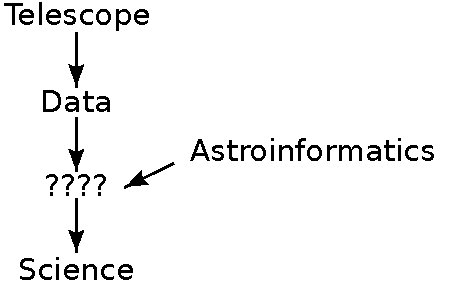
\includegraphics[scale = .8]{astroinformatics}
    \else
    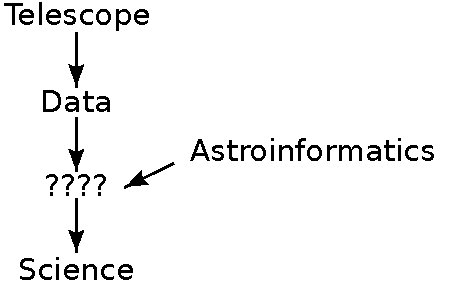
\includegraphics[bb = 92 86 545 742, height=6in]{astroinformatics.png}
    \fi
    \caption{Astroinformatics in the context of astronomy \cite{ballastroinformatics} }
    \label{FigAir}
  \end{center}
\end{figure}
\vspace{-10pt}



The astronomers are not alone and particle physics, biology and other
sciences are also in the vanguard of the data intensive science. This
is great opportunity for interdisciplinary collaboration.

This work deals with the problem of semi-automatic procedures for
finding Be stars \cite{porter2003classical} candidates in the
astronomy surveys. More than straight forward process it's trail and
error approach probing new possibilities with rather interesting than
useful results.

The aim of this work is to be introductory to the technologies of
Virtual Observatory and massive data processing in general.

%  and for this reason it is intended
% to have following properties:

% \begin{itemize}
% \item Main Chapters starts with diagram to ease orietation,
% \item is full of examples, 
% \item is non-linear in nature,
% \item is meant to be compact and consistent,
% \item is far from complete.
% \end{itemize}

\begin{figure}[!htbp]
  \begin{center}
    \leavevmode
    \ifpdf
    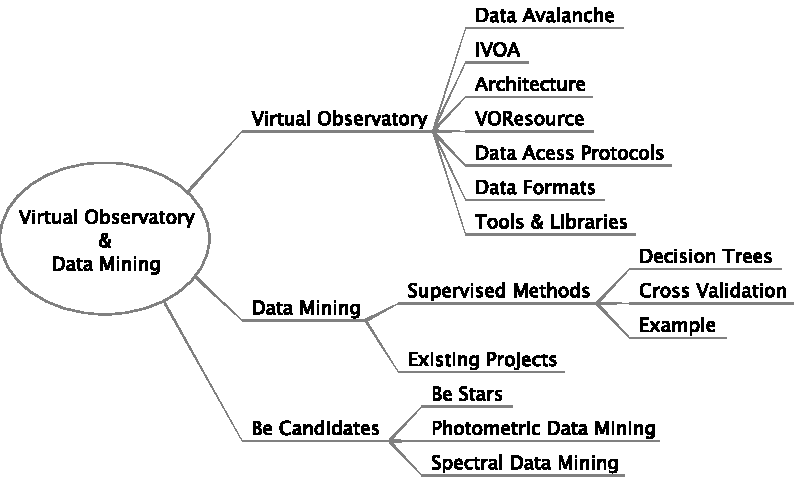
\includegraphics[scale = 1]{mapThesis}
    \else
    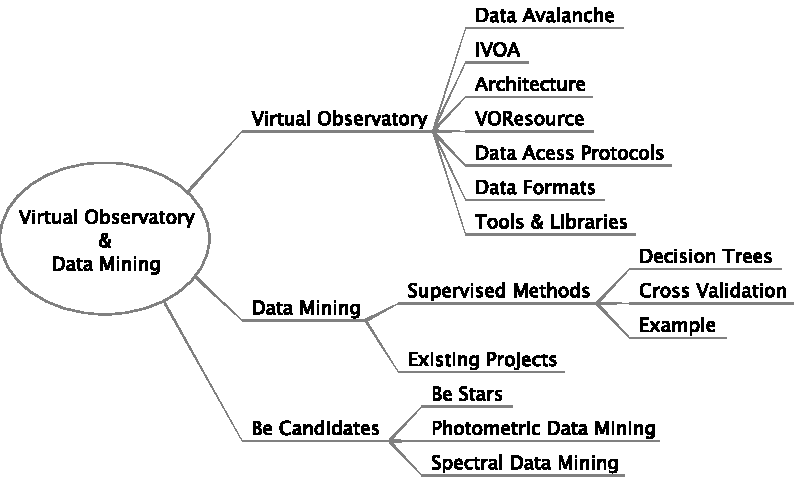
\includegraphics[bb = 92 86 545 742, height=6in]{mapThesis}
    \fi
    \caption{Thesis structure}
    \label{FigStructure}
  \end{center}
\end{figure}


Chapter one is an introduction to the technologies related to Virtual
Observatory. The motivation behind the concept is given without paying
too much attention to historical details. Main principles and
protocols are discussed and explained. Important aspect are
demonstrated on numerous examples. Chapter two is an introduction to
Machine Learning and Data Mining in the context of astrophysics. Only
methods used in practical part of this work are described in detail:
Decision Trees and Support Vector Machines. Examples of several
classifications are demonstrated. Third chapter introduces issues of
Be stars. Chapter Four is practical application of previously
described technologies and methods. Training data of confirmed Be
stars from Ondrejov are correlated with others catalogues to obtain
color indexes and spectra. Results are processed by Data Mining
algorithms using several libraries and tools. In the last chapter
achieved results are critically discussed.

Many scripts were written to achive individual goals. In the text
there are numerous commented snippets of codes. Their purpose is to
demonstrate the concept and they are thefore short and without
auxiliary technicalities such are error handling etc. They are mostly
Python and shell scripts. Any interested person can obtain the full
source codes (including thesis itself) from GIT repository
\footnote{\url{git://github.com/astar/diplomaWork}}.


\begin{table}[ht]
  \centering
  \small
     \begin{tabular}[ht]{l l}
     \toprule
     Name & Description \\
     \midrule
     analyse & Check the wavelength range, raname according to
     target name\\
     getSpectraList & Create SSA Compliant list from\\
     getSpectra & Get spectra links from SSA Server\\
     madmax & Extract feautres from spectra \\
     convolve &  Reduction of Ondřejov's spectra\\
     pf & Print Fits. Shows the spectrum \\
     dm &  Perform classification\\
     makeHTML & Creates HTML pages of results \\ 
     \bottomrule
   \end{tabular}
  \caption{Scripts developed within the scope of the thesis.}
  \label{tab:scripts}
\end{table}


Activities related to this work went beyond this text. Wiki
pages\footnote{\url{http://physics.muni.cz/~vazny/wiki/index.php/Diploma_work}}
were created to present the results and discuss related topic with
supervisor as well as with others scientist around the world. Source
codes were maintained by GIT version system allowing easy sharing. All
software used and produced are open source.






%%% ----------------------------------------------------------------------


%%% Local Variables: 
%%% mode: latex
%%% TeX-master: "../thesis"
%%% End: 


%\pagestyle{fancy}
%\fancyhf{}

% \pagebreak[4]
% \hspace*{1cm}
% \pagebreak[4]
% \hspace*{1cm}
% \pagebreak[4]


\ifpdf
    \graphicspath{{pic/}}
\else
    \graphicspath{{pic/}}
\fi

\chapter{ Virtual Observatory (VO)}

% \begin{lstlisting}[frame=single]
% What is the motivation behind Virtual Observatory? Is data avalanche
% problem only in astronomy? What is IVOA?  What is Virtual Observatory
% architecture?
% \end{lstlisting}

\begin{figure}[!htbp]
  \begin{center}
    \leavevmode
    \ifpdf
    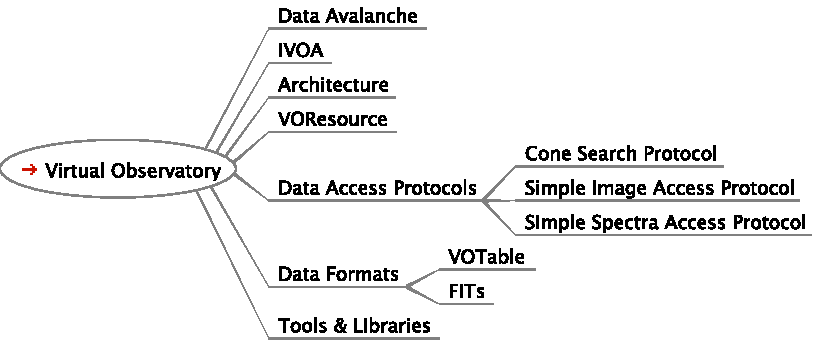
\includegraphics[scale = 1]{mapVirtualObservatory}
    \else
    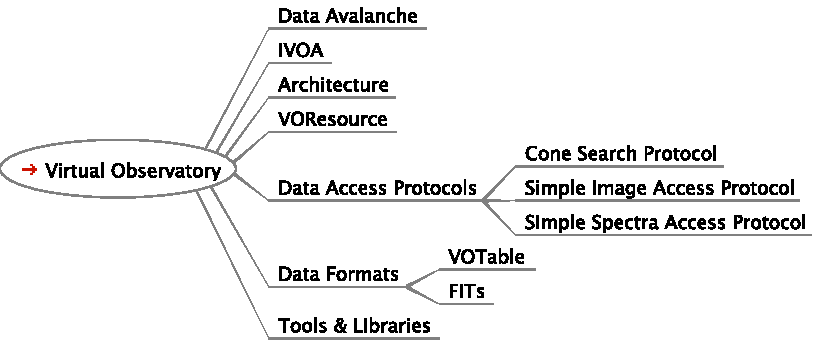
\includegraphics[bb = 92 86 545 742, height=6in]{mapVirtualObservatory}
    \fi
    \caption{Chapter structure}
    \label{FigStructure}
  \end{center}
\end{figure}

\section{ Data avalanche: Opportunity or disaster?}

There are two important trends in current astronomical surveys:

\begin{itemize}

  \item{Size:} The cumulative compressed data holdings of the ESO archive will
    reach 1~Petabyte by 2012 \citep{hanisch2010international}. Projects
    like Large Synoptic Survey Telescope (LSST) will produce about 30
    TB per night, leading to a total database over the ten years of
    operations of 60 PB for the raw data \citep{becla2006designing}.
   
  \item{Complexity:} Modern surveys will cover the sky in different
    wave-bands, from gamma and X-rays, optical, infrared to radio. The
    ability to cross correlate these observations together may lead to
    new understanding of physical
    phenomenas. \citep{hanisch2010international}
\end{itemize}



\noindent Such an amount of data is not possible to transfer over the
network. Data resources are heterogeneous, distributed and
decentralized in their nature.


There is an interesting analogy with the problem (and the solution)
which scientists discovered during LEP project at CERN.  Their problem
was too many documents in different formats. Tim Berners-Lee\footnote{
  Sir Timothy John "Tim" Berners-Lee. British engineer and computer
  scientist and MIT professor credited with inventing the World Wide
  Web.} designed set of protocols (URIs, HTTP and HTML) which allowed
to cross-link and share documents
\citep{berners1990worldwideweb}. This was recognized as generally
useful and World Wide Web was born. An important role in developing
Web standards plays the World Wide Web Consortium
(W3C)\,\footnote{Prior to its creation, incompatible versions of HTML
  were offered by different vendors, increasing the potential for
  inconsistency between web pages.}.
    
    
\section{International Virtual Observatory Alliance (IVOA)}

   \begin{wrapfigure}{r}{0.69\textwidth}
     \vspace{0pt}
     \begin{center}
       \ifpdf
       
\includegraphics[width=0.68\textwidth]{ivoamembers}
       \else
       
\includegraphics[bb = 92 86 545 742, height=6in]{ivoamembers.jpg}
       \fi
     \end{center}
     \vspace{-15pt}
     \caption{IVOA members}
     \vspace{-5pt}
   \end{wrapfigure}


   For handling of heterogeneous distributed data it is necessary to
   have the set of common standards and protocols as well as an
   authority encouraging their implementation. Such an authority is
   the International Virtual Observatory Alliance (IVOA). It currently
   comprises 19~VO programs from Argentina, Armenia, Australia,
   Brazil, Canada, China, Europe, France, Germany, Hungary, India,
   Italy, Japan, Russia, Spain, the United Kingdom, and the United
   States and inter-governmental organizations (ESA and ESO)
   \citep{hanisch2010international}. Standards and specifications
   produced by IVOA can be obtained at \url{http://www.ivoa.net/}.

    %% \begin{figure}[!htbp]
    %%   \begin{center}
    %%     \leavevmode
    %%     \ifpdf
    %%     
\includegraphics[height=6cm]{ivoamembers}
    %%     \else
    %%     
\includegraphics[bb = 92 86 545 742, height=6in]{ivoamembers}
    %%     \fi
    %%     \caption{IVOA members}
    %%     \label{FigAir}
    %%   \end{center}
    %% \end{figure}


\section{Architecture}
    % The Virtual Observatory is the  “middle layer” framework
    % which connects the Resource Layer to the User Layer in a seamless
    % and transparent manner. The objective is to improve and unify access to
    % astronomical data and services.

 
The Architecture is depicted on the figure \ref{FigArchitecture}. The
level of abstraction goes from top to bottom. Starting with
interfaces, used by people or applications to discover resources.  The
next level is the service layer implemented by standard protocols,
followed by the hardware level where actual data are stored. This
onion-like structure hides the complexity of the lower layer and
provide data and meta-data to the higher layer. This concept is
similar to TCP/IP \footnote{TCP/IP (Transmission Control
  Protocol/Internet Protocol).  The basic communication language or
  protocol of the Internet.}  protocol.

    \begin{figure}[!htbp]
      \begin{center}
        \leavevmode
        \ifpdf
        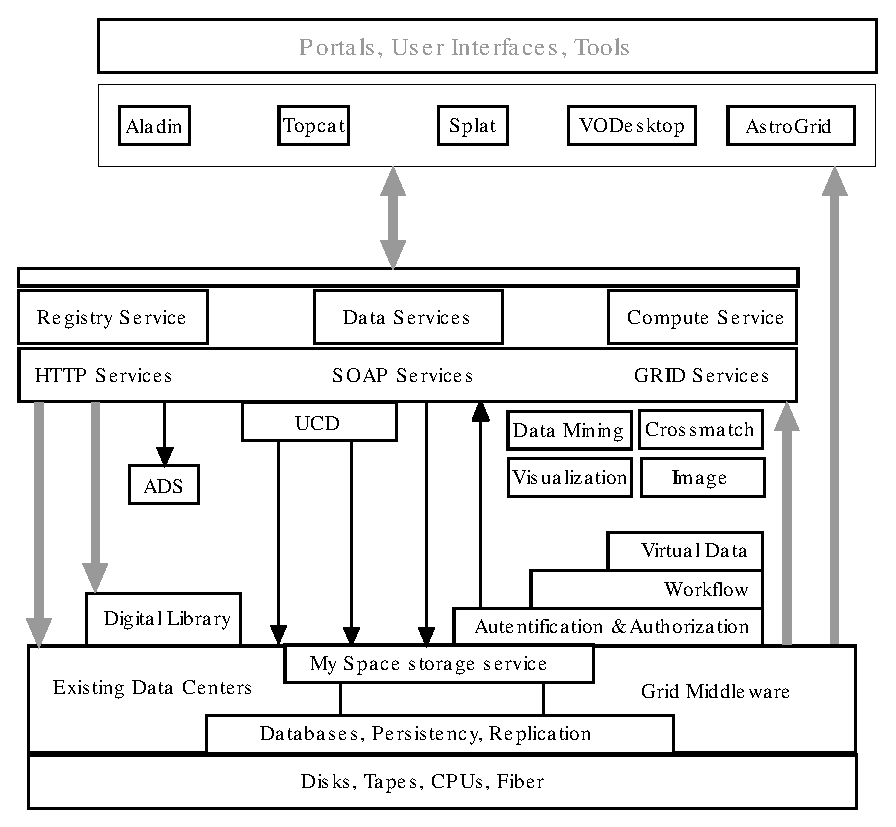
\includegraphics[scale = .8]{architecture}
        \else
        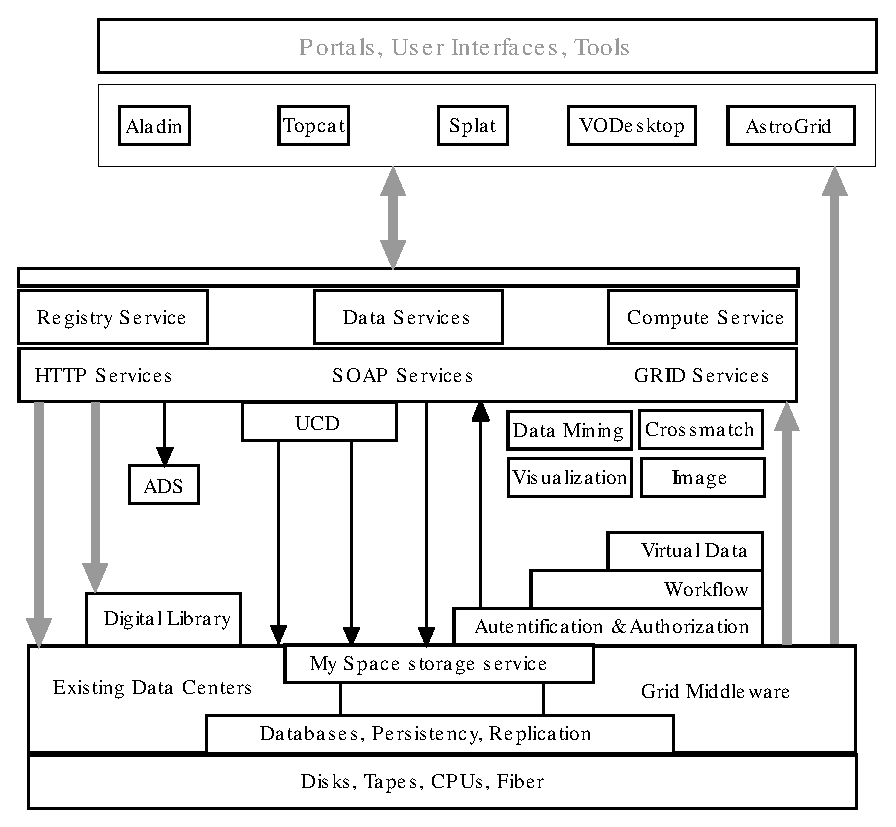
\includegraphics[bb = 92 86 545 742, height=6in]{architecture}
        \fi
      \end{center}
        \caption{VO Architecture}
        \label{FigArchitecture}
    \end{figure}

%\clearpage

    The VO architecture is serviced oriented. Each service is
    autonomous with well defined boundaries. The very important aspect
    of VO implementation is the adoption of formats and protocols used
    in astronomy (FITS) and Computer Science
    (XML\,\footnote{Extensible Markup Language (XML) is a set of rules
      for encoding documents in machine-readable form.} , Web
    Service\,\footnote{method of communication between two electronic
      devices over a network.}  SOAP\,\footnote{Simple Object Access
      Protocol, is a protocol specification for exchanging structured
      information in the implementation of Web Services in computer
      networks.},REST\footnote{Representational State Transfer (REST)
      is a style of software architecture for distributed hyper-media
      systems such as the World Wide Web. Used in
      \url{www.youtube.com} }) for many years. In other words VO does
    not try to reinvent the wheel but it stands on the shoulders of
    giants.

\section{VO Registry}
\noindent 
The VO Registry will allow an astronomer to be able to locate, get
details of, and make use of, any resource located anywhere in the ivo
://space, i.e. in whole Virtual Observatory. The IVOA will define the
protocols and standards whereby different registry services are able
to inter-operate and thereby realize this goal.

\section{VO Resources}
\noindent
A resource is a general term referring to a VO element that can be
described in terms of who curates or maintains it and which can be
given a name and a unique identifier. Just about anything can be a
resource: it can be an abstract idea, such as sky coverage or an
instrumental setup, or it can be fairly concrete, like an organization
or a data collection. \citep{bensonivoa}

The UML\,\footnote{Unified Modeling Language. Standardized
  general-purpose modeling language in the field of object-oriented
  software engineering.}  diagram of the resource is on the figure
\ref{FigResource}. The next paragraph is an attempt to explain this
diagram to non-programmers. Full arrow means generalization. Resource
can be a generalization of organization, data collection, application
or service. Single arrow means association. An organization can be
linked (associated) together with other organization (multiplicity is
represented by number 0,1,\ldots). The same is true for data
collection. Organization is a generalization of and/or provider which
can own zero to N services. The diamond means the aggregation. The
publisher can have any resources.
  
    \begin{figure}[!htbp]
      \begin{center}
        \leavevmode
        \ifpdf
        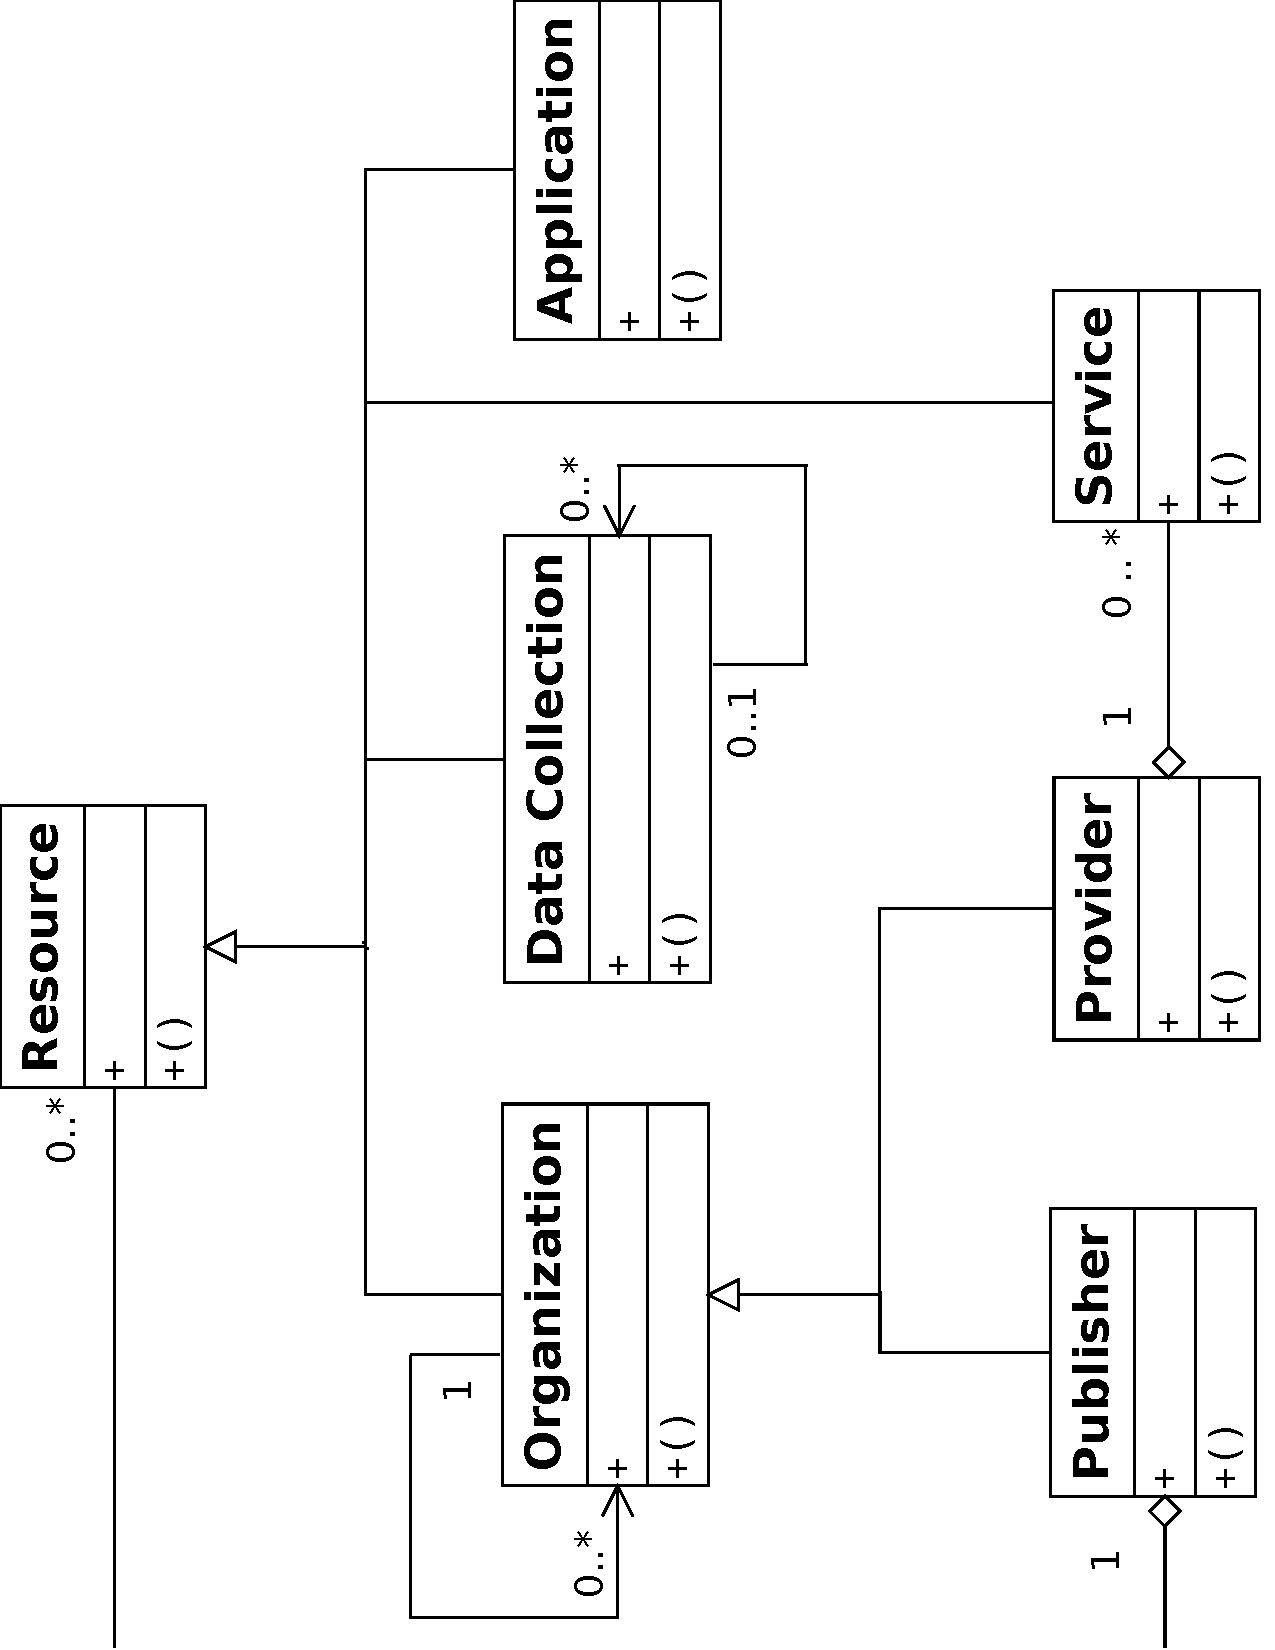
\includegraphics[height=0.8\textwidth, angle=-90]{resources}
        \else
        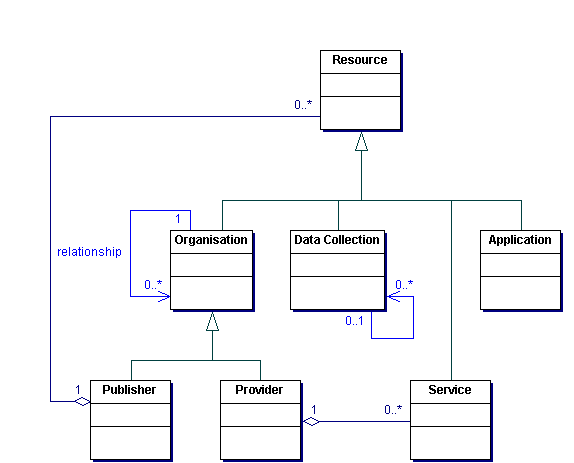
\includegraphics[width=0.9\textwidth]{resource.png}
        \fi
      \end{center}
        \caption{UML diagram of VOResource}
        \label{FigResource}
    \end{figure}

%\clearpage

Following example uses program stilts\footnote{STIL Tool Set. Set of
  command-line tools based on STIL, the Starlink Tables Infrastructure
  Library.} to query registry with parameter shortName equal to
'AIASCR'\footnote{Astronomical Institute of the Academy of Sciences of
  the Czech Republic}. This returns VOTable (see section
\ref{sec:votable}) containing meta-data about the resource.

\begin{lstlisting}[frame=single]
stilts regquery query="shortName like 'AIASCR'"
regurl=http://registry.euro-vo.org/services/RegistrySearch
ofmt=votable-tabledata > resourceExample.vot
\end{lstlisting}

Rows 1--4 define XML and VOTable schema with adequate locations
(xmlns\footnote{XML namespaces. Provide uniquely named elements and
  attributes in an XML document.}) followed by information about the
actual resource. The listing is abbreviated.

  \input{resourceExample.vot}

    
% \section{VOregistry}
%     Is the standard defined by IVOA for registration of VO-Resources

%     The IVOA Registry enables users and applications in the User Layer
%     to discover data and metadata collections, as well services in the
%     Resource Layer.  A resource is a general term referring to a VO
%     element that can be described in terms of who curates or maintains
%     it and which can be given a name and a unique Resource Identifier.
%     A resource can be of various types: a data or metadata collection,
%     a computing or storage element, an application, a data and
%     metadata access service, etc. \citep{gray2007}
    

%     \begin{figure}[!htbp]
%       \begin{center}
%         \leavevmode
%         \ifpdf
%         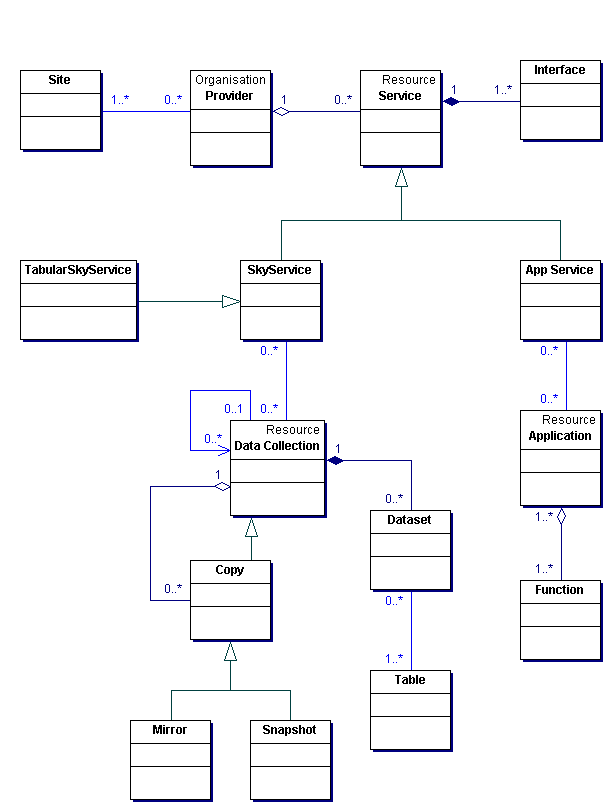
\includegraphics[height=15cm]{registry}
%         \else
%         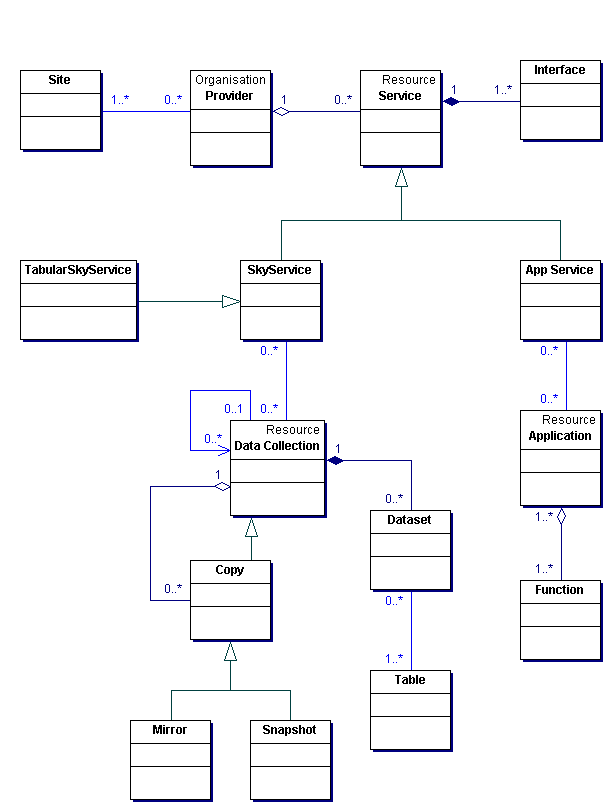
\includegraphics[bb = 92 86 545 742, height=6in]{registry}
%         \fi
%         \caption{UML diagram of VORegistry}
%         \label{FigRegistry}
%       \end{center}
%     \end{figure}


% autonomous, and its boundaries well-defined
% inherently distributed

% picture from
% http://www.ivoa.net/cgi-bin/twiki/bin/view/IVOA/RegistryUseCases

% \clearpage

\section{Data Access Protocols}

Protocols are a very important part of Virtual Observatory. Their
understanding is a key to comprehend the concepts behind VO. They
allow to discover a resource and obtain desirable data. All of them
are based on existing web standards and are designed to be simple and
implement in existing astronomical archives. The main idea is simple
and universal: HTTP GET request with parameters is sent to the
resource and structured document (VOTable) is sent back. There are
many Data Access Protocols like TAP (Table Access Protocol) or SLAP
(Single Line Access Protocol). The most evolved and important for the
practical part of this work are described below.

\subsection{Cone Search Protocol} \label{sec:csp} 

The cone Search was the first standard protocol of Virtual
Observatory. It enables to retrieve records from an astronomical
catalog. The input is the query which describes sky position and the
searched radius on the sky. The output is a list of objects whose
positions lie in the defined vicinity. The output is formatted as a
VOTable. Service compliant with The Cone Search Protocol is called
Cone Search Service. Only the request and response is specified not
the implementation or data storage.


The requirements are:


\begin{enumerate}
\item A respond to a HTTP GET request represented by a URL 

\begin{lstlisting}
  http://<server-address>/<path>?[<extra-GET-arg>&[...]]
\end{lstlisting}

The constrains are expressed as a list of ampersand-delimited GET
arguments. For example:

\begin{lstlisting}
  http://simbad.u-strasbg.fr/simbad-conesearch.pl?RA=24.5&DEC=-57.2&SR=0.1
\end{lstlisting}

Where RA is right-ascension, DEC declination and SR the searched
radius of the cone in the ICRS coordinate system in decimal
degrees. These parameters are required, others are optional.

\item A return an XML document in the VOTable format.

  There are several requirements on the contents of the table:

  \begin{itemize}
  \item UCD fields "ID\_MAIN", "POS\_EQ\_RA\_MAIN", "POS\_EQ\_DEC\_MAIN" must
    be present.
  \item Return VOTable with single PARAM element name="Error" in the
    case of error.
  \end{itemize}

\end{enumerate}

Cone Search is implemented in many software packages. Besides standard
VO tools like TOPCAT or STILTS also in MUNIPACK and many others.
Following example shows simple query to SIMBAD \citep{wenger2000simbad}
catalog using method \emph{urlopen} of Python library \emph{urllib2}.
 
\begin{lstlisting}
  import urllib2
  response = urllib2.urlopen('http://simbad.u-strasbg.fr/simbad-conesearch.pl?RA=24.5&DEC=-57&SR=0.1')
  print response.read()
\end{lstlisting}

\noindent The same result can be obtained using program like wget\footnote{program
  for non-interactive download of files from the Web} or Web browser.

\subsection{Simple Image Access Protocol}
The key idea behind the SIA Protocol is to allow users and programs to
retrieve images created by an image service on-the-fly. From technical
point of view it is designed in a similar way as Cone Search Protocol
(see section \ref{sec:csp}), specifically as name-value HTTP GET
requests and the VOTable XML format output. The user specifies ideal
image coverage (position and the size) he wants to receive and the
image service produces a list of images it can return in the VOTable
format. The user then could issue getImage request to retrieve
desirable images.

There are following requirements for compliance. A SIA service must
support:

\begin{itemize}
\item Image Query web method,
\item Image Retrieval (getImage) web method.
\end{itemize}

\noindent Other optional services may be provided by servers: 

\begin{itemize}
\item Image Cutout Service.

  Provides rectangular regions of large images.
\item Image Mosaicing Service.

  Size, scale and projection could be specified.
\item Atlas Image Archive

  Pre-computed atlas of images.
\item Pointed Image Archive.  

  Images are not part of a sky survey but
  rather focused on specific source
\end{itemize}


To get a list of images query has to sent via HTTP GET method. The
first part is base URL. The second part are parameters specifying
image properties such as position (POS), size of searched radius
(SIZE), etc.

\begin{lstlisting}
  http://<server-address>/<path>?[<extra GET arg>&[...]]
\end{lstlisting}

There are two examples of using SIA protocol to obtain image. First
one from SDSS, second from Hubble Space Telescope archive. 

\begin{lstlisting}
  http://skyview.gsfc.nasa.gov/cgi-bin/vo/sia.pl?SURVEY=SDSS&POS=18.87667,-0.86083&SIZE=1
  http://hubblesite.org/cgi-bin/sia/hst_pr_sia.pl?POS=83.6,22.0&SIZE=1.0
\end{lstlisting}

There is more complex example using the Astrogrid framework to show
how to discover SIA service and obtain an image. First registry method
searchSiap is used to find SIA service for SDSS, this is then used in
SiapSearch method to obtain result in VOTable format.

\begin{lstlisting}
  In [1]: from astrogrid import Registry, ConeSearch
  In [2]: list = reg.searchSiap('SDSS')
  In [3]: print [p['id'] for p in list]
  -------> print([p['id'] for p in list])
  ['ivo://nasa.heasarc/skyview/sdss']
  
  In [4]: siap = SiapSearch('ivo://nasa.heasarc/skyview/sdss')
  In [5]: result = siap.execute(18.8, -0.8, 1.0)
\end{lstlisting}

% Even more sophisticated example is described below. The STILTS tool is
% used to get images from 2MASS survey for many objects from the file
% using SIA protocol. This file is the list of Be starts from Ondrejov
% used later in this work.


 

\subsection{Simple Spectra Access Protocol}

SSA Protocol allows to discover and obtain 1-D spectra from VO
Service. It shares many similarities with the previously discussed SIA
Protocol. It defines a uniform interface to remotely discover and
access simple 1-D spectra.

\noindent The process to obtain a spectrum consists of following steps:

\begin{itemize}
\item Query the resource registry.
\item Data discovery of selected services to get available spectra in
  VOTable format.
\item Download selected spectra using URL.
\end{itemize}

\noindent The spectra could be one of the following types:

\begin{itemize}
\item Observed spectra.
\item Theoretical spectra.
\end{itemize}

\noindent To be a SSA-compliant, the service must provide:

\begin{enumerate}
\item HTTP GET interface, understanding at least parameters POS, SIZE,
  TIME (time and date of exposure), BAND (spectral range covered) and
  returning the query response encoded as a VOTable document.
\item GetData method returning data in at least one of the
  SSA-compliant data formats (VOTable, FITS)
\item FORMAT=METADATA metadata query feature
\end{enumerate}


Following example show how to discover resources with SSA capability
using STILTS program. 

\begin{lstlisting}
  stilts regquery query="shortName like 'ESO' capability/@standardID =
  'ivo://ivoa.net/std/SSA'" ocmd="keepcols 'ShortName accessUrl'"
  ofmt=ascii
\end{lstlisting}

With information of service URL, one can specify a query to obtain a
list with available spectra in VOTable format. This can be used in Web
browser or via programs such \emph{wget} or \emph{curl}.

\begin{lstlisting}
  http://archive.eso.org/apps/ssaserver/EsoProxySsap?REQUEST=queryData&POS=83.63,22&SIZE=1
\end{lstlisting}

\section{Data Formats}
Astronomy has always been in forefront of image producing and
processing. This is especially true for the era of digitization. The
situation with data formats in astronomy is unique. There are just few
very good standards with variety of implementation in many programming
languages. Virtual Observatory takes advantage of this heritage and
implements these formats in a sensible way into its own standards.
 
\subsection{VOTable}
\label{sec:votable}
\subsubsection*{Motivation}
VOTable is an flexible storage and exchange format fundamentally
interconnected with Virtual Observatory. It has features for big-data
and Grid computing. Data can be stored in the different ways in
dependence of their nature and size. Small tables can be stored in
pure XML\,\footnote{Extensible Markup Language. W3C standard. Set of
  rules for encoding documents in machine-readable form}, while
large-scale data can be referenced with the URL\,\footnote{Uniform
  Resource Locator. Uniform Resource Identifier (URI) that specifies
  where an identified resource is available and the mechanism for
  retrieving it.} syntax protocol://location.  It combines web
standards (it is based on XML) and astronomy tradition in storing data
(it is FITS compatible). The expiration and the authentication are
also supported.

\subsubsection*{Structure}
Following example of VOTable was created from SDSS FITS file used in
this work. First there is an information about XML and VOTable
versions and references to corresponding XML Schema \footnote{Define
  the legal building blocks of an XML document.}. \textrm{TABLE} tag
encapsulates tabular data. \textrm{FIELD} tag describes identification
(ID), type and precision of columns. \textrm{DATA} tag contains data
(here) in TABLEDATA format (other types are FITS and BINARY).
 
\begin{lstlisting}
<?xml version="1.0" encoding="utf-8"?>
<!-- Produced with vo.table version 0.6
     http://www.stsci.edu/trac/ssb/astrolib
     Author: Michael Droettboom <support@stsci.edu> -->
<VOTABLE version="1.0"
 xmlns:xsi="http://www.w3.org/2001/XMLSchema-instance"
 xsi:noNamespaceSchemaLocation="http://www.ivoa.net/xml/VOTable/v1.0"
 xmlns="http://www.ivoa.net/xml/VOTable/v1.0">
 <RESOURCE type="results" >
  <TABLE >
   <FIELD ID="col0" name="wave" datatype="float" unit=""
   precision="F9"/>
  <DATA>
    <TABLEDATA>
     <TR>
      <TD>4012.50757</TD>
     </TR>
 </TABLEDATA>
   </DATA>
  </TABLE>
 </RESOURCE>
</VOTABLE>
\end{lstlisting}


\subsubsection*{Examples}
All examples were created using ATpy\,\footnote{High-level Python
  package providing a way to manipulate tables of astronomical data in
  a uniform way.}. Following example shows transformation of FITS into
VOTable.

\begin{lstlisting}
  In [1]: import atpy
  In [2]: tbl = atpy.Table('spSpec-53401-2052-458.fit',hdu=1)
  Auto-detected input type: fits
  In [3]: tbl.write('votableExample.xml')
  Auto-detected input type: vo
\end{lstlisting}

\subsection{FITS}
\subsubsection*{Motivation}
\emph{
"An archival format must be utterly portable and self-describing, on
the assumption that, apart from the transcription device, neither the
software nor the hardware that wrote the data will be available when
the data are read."} \citep{nrc1995}


\bigskip

FITS (Flexible Image Transport System) was originally created for data
exchange between WSRT\,\footnote{Westerbork Synthesis Radio Telescope}
and the VLA \footnote{Very Large Array} \citep{fits1997}. It is now
used as a file format to store, transmit, and manipulate scientific
data and it is (thanks to it's revolutionary design) de facto standard
in astronomy.


\subsubsection*{Structure}

A FITS file can contain several HDUs (Header and Data Units). The
first part of each HDU is the header, composed of ASCII card images
containing \textrm{keyword=value} statements that describe the size,
format and structure. A FITS file shall be composed of the following
FITS structures, in the order listed:

\begin{itemize}
\item Primary header and data unit (HDU).
\item Conforming Extensions (optional).
\item Other special records (optional, restricted).
\end{itemize}


Standards and documents related to FITS are maintained by IAU-FWG
\footnote{International Astronomical Union FITS Working Group.} and
available at \url{http://fits.gsfc.nasa.gov}.

\subsubsection*{Examples}

There are many libraries for working with FITS files. The official
list is available at
\url{http://fits.gsfc.nasa.gov/fits_libraries.html}. PyFITS, library
for Python programming language was used for following
examples. PyFITS is a development project of the Science Software
Branch at the Space Telescope Science Institute
\url{http://www.stsci.edu/resources/software_hardware/pyfits}.


Reading FITS headers.

\begin{lstlisting}
In [1]: import pyfits
In [2]: hdulist = pyfits.open('spSpec-53237-1886-248.fit')
In [3]: hdulist.info()
Filename: spSpec-53237-1886-248.fit
No.    Name         Type      Cards   Dimensions   Format
0    PRIMARY     PrimaryHDU     213  (3874, 5)     float32
1                BinTableHDU     54  6R x 23C      [1E, 1E, ...
2                BinTableHDU     54  44R x 23C     [1E, 1E, ...
3                BinTableHDU     18  1R x 5C       [1E, 1E, ...
\end{lstlisting}

\noindent Printing primary HDU.

\begin{lstlisting}
In [4]: print hdulist[0].header
-------> print(hdulist[0].header)
DATE-OBS= '2004-08-20'         / 1st row - TAI date                             
TAIHMS  = '10:36:18.11'        / 1st row - TAI time (HH:MM:SS.SS) (TAI-UT = appr
TAI-BEG =        4599713999.00 / Exposure Start Time                            
TAI-END =        4599717089.00 / Exposure End Time                              
MJD     =                53237 / MJD of observation                             
MJDLIST = '53237   '           /                                                
VERSION = 'v3_140_0'           / version of IOP                                 
TELESCOP= 'SDSS 2.5-M'         / Sloan Digital Sky Survey
\end{lstlisting}

Updating FITS file.

\begin{lstlisting}
  In [1]: prihdr = hdulist[0].header
  In [2]: prihdr.update('observer', 'Astar')
  In [3]: prihdr.add_history('I updated this file 3/27/11')
\end{lstlisting}

\section{VO Tools \& Libraries}
There are many programs and libraries allowing user to interact with
VO services. Such application is called to be VO-enabled. Thanks to
the openness and the standardization anyone can develop his own
application or enable existing\footnote{For example Astroweka or
  Mirage.} application to interact with VO Services. Libraries are
also available for many programming languages enabling advanced users
to interact with VO from scripts and programs. A such diversity is
healthy and probably the only possible way to ensure natural evolution
of Virtual Observatory.
% This chapter describes some of the libraries and applications ued during
% this work. Low level tools and libraries are stressed as opposite to
% standard introductory texts of Virtual Observatory where the focus is
% on "user friendly" GUI applications.

Every VO-enabled application can communicate with each other by
sending messages and data (e.g. in VOTable format) by protocols
PLASTIC and SAMP. It enables to create complex analysis systems by
chaining individual components.

% \subsection{Command line tools}
% \subsubsection*{Astro Runtime}

% middleware that makes it simple to call Virtual Observatory services
% from any programming language
% \subsection{GUI Appliactions}


% Example from program pf (plot fits) created for purposes of this work
% to plot $H\alpha$ emission in the spectra.

% \begin{lstlisting}
%  def read(file):
%     """ Read fits file. Convert wavelength to angstroms """ 
%     data = pyfits.getdata(file)
%     w = lambda x : 10.0**(3.5796 + x*10.0**(-4))
%     x = np.arange(1,data[0].size + 1)
%     xx  = w(x) # convert to actual wavelenght
%     return np.asarray([xx, data[0]])

%  def plot(file,xdata,ydata,spLine):
%     fig = plt.figure()
%     ax = fig.add_subplot(111)
%     graph = ax.plot(xdata,ydata, 'r')
%     ax.set_title(file)
%     ax.set_xlabel("$Wavelenght [\\,\textrm{\AA}]$")                                                                            
%     ax.set_ylabel("$Energy [10^{-17} erg/s/cm^2/\\,\textrm{\AA}]$")
%     ax.axvline(x=spLine, color = 'g', ls ='--')
% \end{lstlisting}







%% \section{First Paragraph}
%% And now I begin my first chapter here ...

%% Here is an equation\footnote{the notation is explained in the nomenclature section :-)}:
%% \begin{eqnarray}
%% CIF: \hspace*{5mm}F_0^j(a) &=& \frac{1}{2\pi \iota} \oint_{\gamma} \frac{F_0^j(z)}{z - a} dz
%% \end{eqnarray}
%% \nomenclature[zcif]{$CIF$}{Cauchy's Integral Formula}                                % first letter Z is for Acronyms 
%% \nomenclature[aF]{$F$}{complex function}                                                   % first letter A is for Roman symbols
%% \nomenclature[gp]{$\pi$}{ $\simeq 3.14\ldots$}                                             % first letter G is for Greek Symbols
%% \nomenclature[gi]{$\iota$}{unit imaginary number $\sqrt{-1}$}                      % first letter G is for Greek Symbols
%% \nomenclature[gg]{$\gamma$}{a simply closed curve on a complex plane}  % first letter G is for Greek Symbols
%% \nomenclature[xi]{$\oint_\gamma$}{integration around a curve $\gamma$} % first letter X is for Other Symbols
%% \nomenclature[rj]{$j$}{superscript index}                                                       % first letter R is for superscripts
%% \nomenclature[s0]{$0$}{subscript index}                                                        % first letter S is for subscripts

%% \section{Second Paragraph}
%% and here I write more ...\citep{texbook}

%% \subsection{sub first paragraph}
%% ... and some more ...

%% Now I would like to cite the following: \citep{latex} and \cite{texbook}
%% and \citep{Rud73}.

%% I would also like to include a picture ...

%% \begin{figure}[!htbp]
%%   \begin{center}
%%     \leavevmode
%%     \ifpdf
%%       \includegraphics[height=6in]{aflow}
%%     \else
%%       \includegraphics[bb = 92 86 545 742, height=6in]{aflow}
%%     \fi
%%     \caption{Airfoil Picture}
%%     \label{FigAir}
%%   \end{center}
%% \end{figure}

%% % above code has been macro-fied in Classes/MacroFile.tex file
%% %\InsertFig{\IncludeGraphicsH{aflow}{6in}{92 86 545 742}}{Airfoil Picture}{FigAir}

%% So as we have now labelled it we can reference it, like so (\ref{FigAir}) and it
%% is on Page \pageref{FigAir}. And as we can see, it is a very nice picture and we
%% can talk about it all we want and when we are tired we can move on to the next
%% chapter ...

%%I would also like to add an extra bookmark in acroread like so ...
% \ifpdf
%   \pdfbookmark[2]{bookmark text is here}{And this is what I want bookmarked}
% \fi
% ------------------------------------------------------------------------


%%% Local Variables: 
%%% mode: latex
%%% TeX-master: "../thesis"
%%% End: 

%\chapter{Data Mining}
Virtual Observatory may be seen as data infrastructure. It enables
astronomers to get data more easily in a uniform way. But there is
another and even bigger problem now. How to deal with such amount of
data? Can we change the problem to opportunity? Can we discover new
phenomena, new types of objects or exploit natural groups in the data?
Data Mining and related techniques are created exactly for such
purposes. Used correctly, it can be powerful approach, promising
scientific advance. On the other side this field is very complex with
dozens of different methods and algorithms. This forms needs and
opportunity for interdisciplinary cooperation with Data Mining
experts. This can be very beneficially for both fields, providing
astronomers with interesting methods for data analysis and computer
scientist with large ammout of quality data.

\section{Supervised Methods}
These methods are also known as predictive\cite{ball2010data}. They
rely on training set with known target property. This set must be
representative. The selected method is trained on that set and the
result is then used on data for which the target property is not
known. Among supervised method are classification, regression, anomaly
detection and others.

\subsection{Decision Tree (DT)}
Is an example of supervised classification. Based on final number of
data $(x^{(1)},\ldots,x^{(p)})$ with known class $C_1,\ldots, C_m$
classifier is created, i.e. image $f$ classifying any $x \in
\mathcal{X}, f:\mathcal{X}\rightarrow \mathcal{Y}$, where
$\mathcal{X}$ is a set of possible input vectors and $\mathcal{Y}$ is
a set which values represents classes $C_1,\ldots, C_m$ (for example
$\mathcal{Y} = {1,\ldots,m}$). The model is consctructed based on
traning set as a tree structure, where leaves represent
classifications and branches conjunctions of features that lead to
those classifications. The main advatages of DT are:

\begin{itemize}
\item Simple to understand and interpret.
\item Able to handle both numerical and categorical data.
\item Uses a white box model.
\item Perform well with large data in a short time.
\end{itemize}

In pseudocode, the general algorithm for building decision trees is
\cite{kotsiantis2007supervised}:
\begin{enumerate}
\item Check for base cases
\item For each attribute a
  \begin{itemize}
  \item Find the normalized information gain from splitting on a
  \end{itemize}
\item Let "a best" be the attribute with the highest normalized information gain
\item Create a decision node that splits on "a best"
\item Recur on the sublists obtained by splitting on "a best", and add
  those nodes as children of node
\end{enumerate}

Furtheremore algoritms C4.5 is described for several reasons: Its code
is aviable and free implementeations exist (J48 in weka), is de-facto
standard in classsifiction using DT, is used in practical part of this
work. The key question of DT algoritm is how to choose attribute for
splitting the tree. C4.5 Uses meassures based on information entropy:

\begin{equation}
  \label{eq:entropy}
  H(X) = -\sum_{i=1}^n {p(x_i) \log_2 p(x_i)},
\end{equation}
where $p(x_i)$ is probability of occurrence of class $i$ and $n$ is the
number of classes.

After the tree is created it is optimized by pruning, which prevent
over-fitting.

%\subsubsection{Pruning}         
\subsubsection{Cross-validation}
The quality of the training set is crucial to good results. The amount
of data for testing is always limited. In general, one cannot be sure
whether a sample is representative. If for example certain group is
missing, one could not expect a classifier learned from such data to
perform well on the examples s of that class. One of the technique used
here is cross-validation.

The data is divided into fixed number of partitions and each in turn
is used for testing and the reminder is used for training. Finally,
the number of partitions error estimates are averaged to yield an
overall error. The standard is to used 10-fold cross-validation. This
number is a result of tests on numerous data sets \cite{witten2005data}

\subsubsection{Example: Classifying Galaxies Stars and QSO}
There is an example of classifying Galaxies Stars and QSO based on
photometric properties using Decision Tree algorithm J48 (C4.5 in
Weka). The data are from SDSS (Sloan Digital Sky Survey) DR7. 298
Objects were used (100 Stars, 99 Galaxies, 99 QSO). SDSS Filters
u,g,r,i were used as parameters. Data were obtained using SQL query
from SDSS CAS.

\begin{lstlisting}
SELECT TOP 100 u-g,g-r,r-i,s.specClass
FROM PhotoPrimary p join SpecPhotoAll s on p.objid=s.objid 
WHERE s.specClass in (1)
AND u between 18 and 19
UNION all
SELECT top 100 u-g,g-r,r-i,s.specClass
FROM PhotoPrimary p join SpecPhotoAll s on p.objid=s.objid 
WHERE s.specClass in (2)
AND u between 18 and 19
UNION all
SELECT top 100 u-g,g-r,r-i,s.specClass
FROM PhotoPrimary p join SpecPhotoAll s on p.objid=s.objid 
WHERE s.specClass in (3)
AND u between 18 and 19
\end{lstlisting}

The following listing shows the result of classification. The
classifier was able to distinguish 95\% of the processed objects.

\begin{table}[ht]
  \centering
  \small
     \begin{tabular}[ht]{l r@{,}l r@{,}l l l}
     \toprule
     Filter & Wavelength [$\AA$] \\
     \midrule
     Ultraviolet (u) & 3543 \\
     Green (g) & 4770\\
     Red (r) & 6231\\
     Near Infrared (i) & 7625\\
     Infrared (z) & 9134 \\
     \bottomrule
   \end{tabular}
  \caption{SDSS Filters}
  \label{tab:SDSSFilter}
\end{table}


\begin{lstlisting}
Correctly Classified Instances          96               95.0495 %
Incorrectly Classified Instances         5                4.9505 %
Kappa statistic                          0.9257
Mean absolute error                      0.0669
Root mean squared error                  0.1778
Relative absolute error                 15.0587 %
Root relative squared error             37.6973 %
Total Number of Instances              101     
\end{lstlisting}

The big advantage of Decision Trees over black box algorithms (such as
Neural Network) is that one could understand the classification
process. The decision tree generated for this example is following:

\begin{lstlisting}
  ug <= 0.663668
|   gr <= -0.191208: 1 (7.0)
|   gr > -0.191208: 3 (104.0/5.0)
ug > 0.663668
|   ri <= 0.285854: 1 (88.0/5.0)
|   ri > 0.285854
|   |   ri <= 0.314657
|   |   |   gr <= 0.692108: 2 (6.0)
|   |   |   gr > 0.692108: 1 (3.0)
|   |   ri > 0.314657: 2 (90.0/2.0)
\end{lstlisting}

Useful tool for understanding how classifier was successful on
individual classes is the confusion matrix. Columns shows how the
object was classified and the row what is his actual class. In this
example QSO were classified correctly in 100\% cases. Distinction
between stars and galaxies are a bit worse and the algorithm classify 2
galaxies incorrectly as stars and two stars were confused with
galaxies. On stars was incorrectly classified as QSO.
 
\begin{lstlisting}
  s  g  q   <-- classified as
 30  2  1 |  s 
  2 33  0 |  g 
  0  0 33 |  q 
\end{lstlisting}

\begin{figure}[!htbp]
%      \begin{center}
        \leavevmode
        \ifpdf
        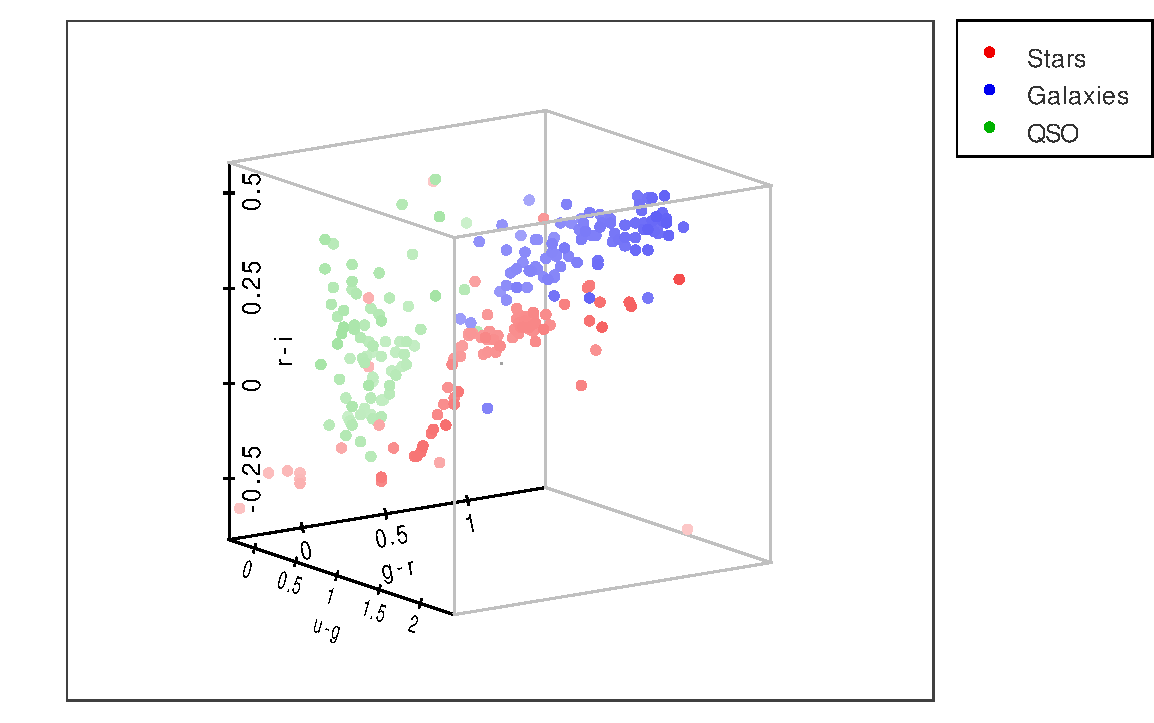
\includegraphics[scale = .7]{starsGalaxiesQSO}
        \else
        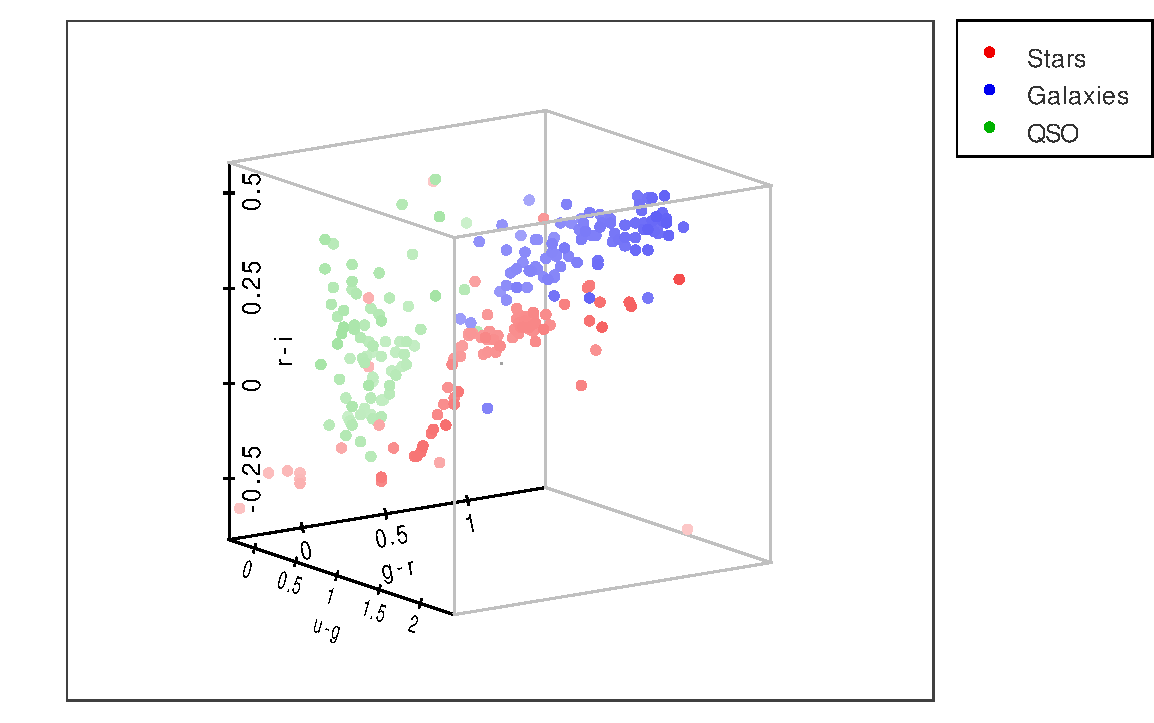
\includegraphics[bb = 92 86 545 742, height=6in]{starsGalaxiesQSO}
        \fi
        \caption{Color Diagram of the problem. It shows that individual
        objects classes occupies different region in the digram.}
        \label{FigStarsGalaxiesQSO}
 %     \end{center}
\end{figure}

\clearpage


\subsection{Support Vector Machine (SVM)}

\section{Unsupervised Methods}
\section{Existing Projects}
\subsection{Weka}
\subsection{SVM lib}
\subsection{DAME}
%\chapter{Be candidates}
Astronomical objects used in this work to demonstrate some of the
discussed technologies and methods were Be stars. The target was to
develop a process of finding new candidates in the available
data. Several approaches were considered and two of them are discussed
in the rest of this text. First one utilizes photometric properties
of Be stars, second uses spectra characteristics.


\section{Be stars}

"Classical Be stars are B-type stars close to the main sequence that
exhibit line emission over the photometric spectrum. The excess is
attributed to a circumstellar gaseous component that is commonly
accepted to be in the form of an equatorial disk."

\cite{porter2003classical}.

    \begin{figure}[!htbp]
      \begin{center}
        \leavevmode
        \ifpdf
        \subfloat{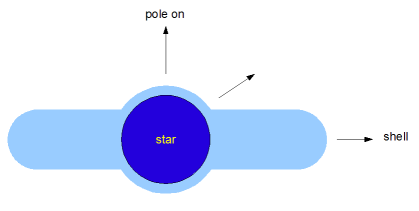
\includegraphics[width=0.5\textwidth]{beStar2}}                
        \subfloat{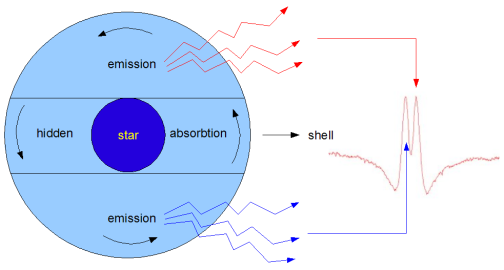
\includegraphics[width=0.5\textwidth]{beStar1}}
        \else
        \includegraphics[bb = 92 86 545 742, height=6in]{beStar}
        \fi
        \caption{Model of a typical Be star \cite{hirata1984star}}
        \label{Figjhk_be_b}
      \end{center}
    \end{figure}

    \begin{figure}[!htbp]
      \begin{center}
        \leavevmode
        \ifpdf
        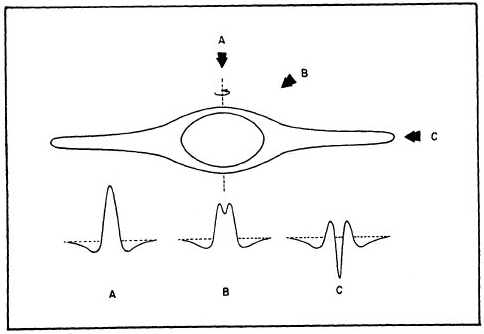
\includegraphics[scale =1]{beSpectra}
        \else
        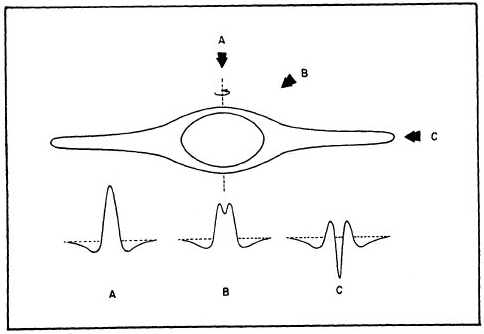
\includegraphics[bb = 92 86 545 742, height=6in]{beSpectra}
        \fi
        \caption{Example of spectra of Be stars based on view angle
          \cite{slettebak1988stars}}
        \label{Figjhk_be_b}
      \end{center}
    \end{figure}

\clearpage

\section{Photometric Data Mining}

% The question I have tried to answer in this chapter was: Is it
% possible to find Be stars candidates based on photometric properties
% only? To answer this question I needed training set of confirmed Be
% stars, set of non Be stars (spectral type B was considered) and some
% Data Mining algorithm to perform classification.

Classification based on photometric properties is very attractive from
several points of view. There are much more aviable phometric then
spectral data and they are easier accesiable. Because they are easier
to gain the disproportion between photometric and spectral data will
probably increase in the future as well. The distinction between Be
and other types of stars also should be theoretically possible since
the Be stars exibits infrared excess correlated to the H$\alpha$
emission \cite{van1995halpha}.

\subsection{Data preprocessing}

I was provided by a list of confirmed Be stars from Academy of Science
Ondřejov. This list consist of 625 manually chosen objects. Data were
correlated with Hipparcos \cite{perryman1997hipparcos} catalog to
obtain RA, DEC and then with 2MASS\cite{2006AJ131.1163S} catalog to
obtain J,H,K Colors using method of multi-cone search in Virtual
Observatory. The second set was acquired from Hipparcos catalog using
following SQL query:

\begin{lstlisting}
  Select * 
  From maincat as m, hipva1 as h 
  Where  (m.HIP=h.HIP )  
  And h.SpType Like 'B%'
\end{lstlisting}

The result was cross-correlated with 2MASS catalog to obtain the same
colors as for the confirmed Be stars. Color digram of this two sets
are on the figure \ref{Figjhk_be_b}

    \begin{figure}[!htbp]
      \begin{center}
        \leavevmode
        \ifpdf
        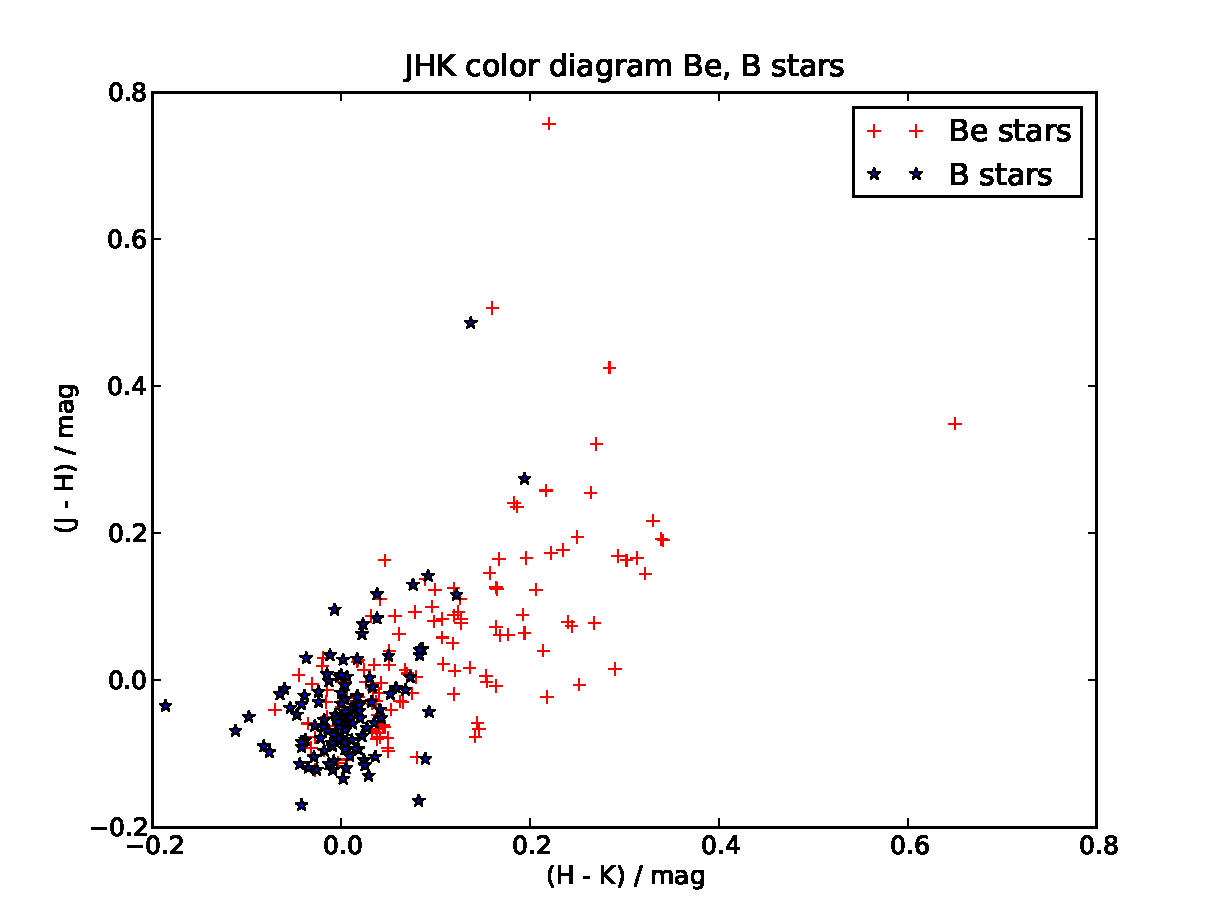
\includegraphics[scale =.6]{jhk_be_b}
        \else
        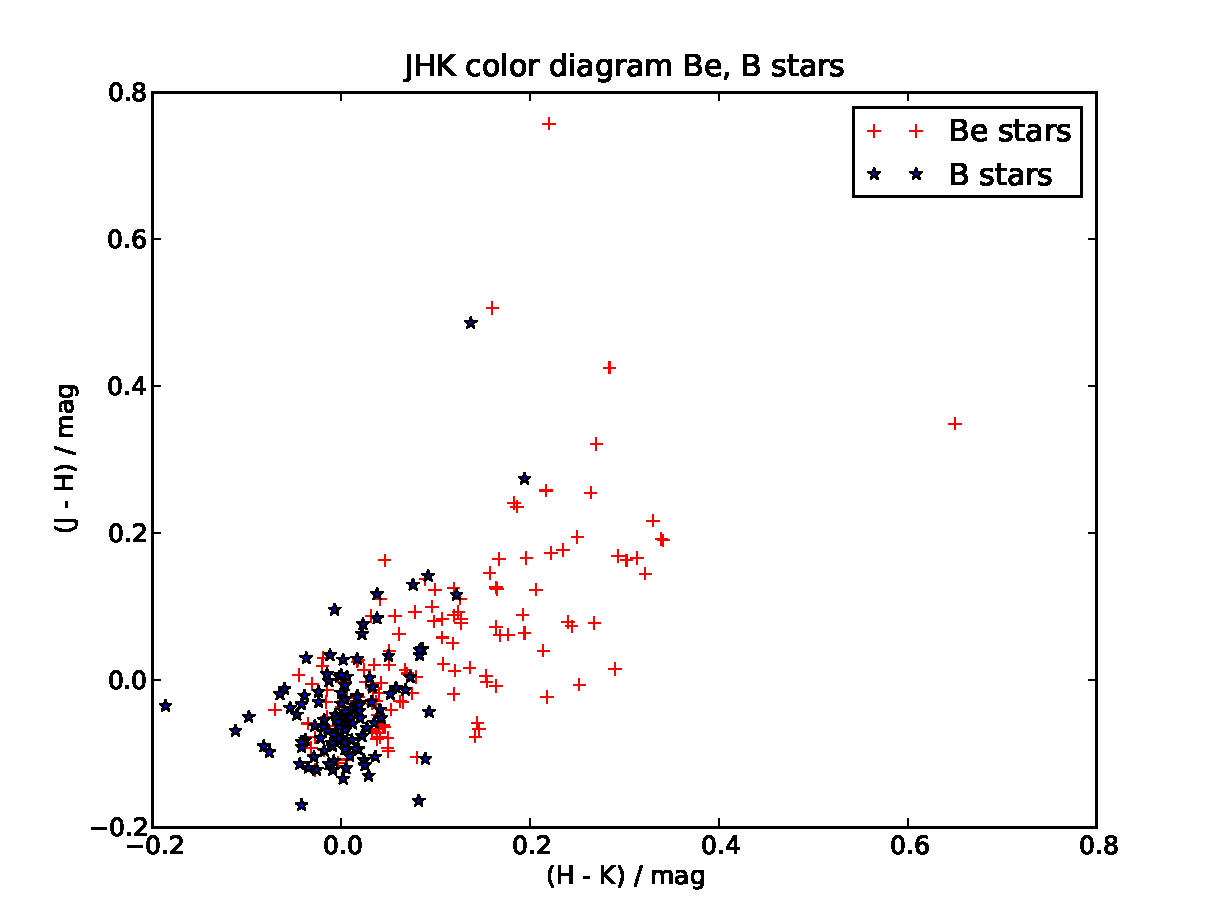
\includegraphics[bb = 92 86 545 742, height=6in]{jhk_be_b}
        \fi
        \caption{Color diagram of confirmed Be stars Vs B stars}
        \label{Figjhk_be_b}
      \end{center}
    \end{figure}

    The uncertainties were computed for each object using propagation
    of error. These errors and depicted on the figure
    \ref{Figjhk_be_b_errors}. Although the uncertainties are
    significant certain trends are presented.

\begin{align*}
  \delta_{(j - h)} = \sqrt{\left(\frac{\partial(j - h) }{\partial
        j}\right)^2\delta_j^2 + \left(\frac{\partial(j - h) }{\partial
        h}\right)^2\delta_h^2} \\
  \frac{\partial(j - h) }{\partial j } = 1,\frac{\partial(j - h)
  }{\partial h } = -1 \\
  \delta_{(j - h)} = \sqrt{\delta_j^2 + \delta_h^2}
\end{align*}


    \begin{figure}[!htbp]
      \begin{center}
        \leavevmode
        \ifpdf
        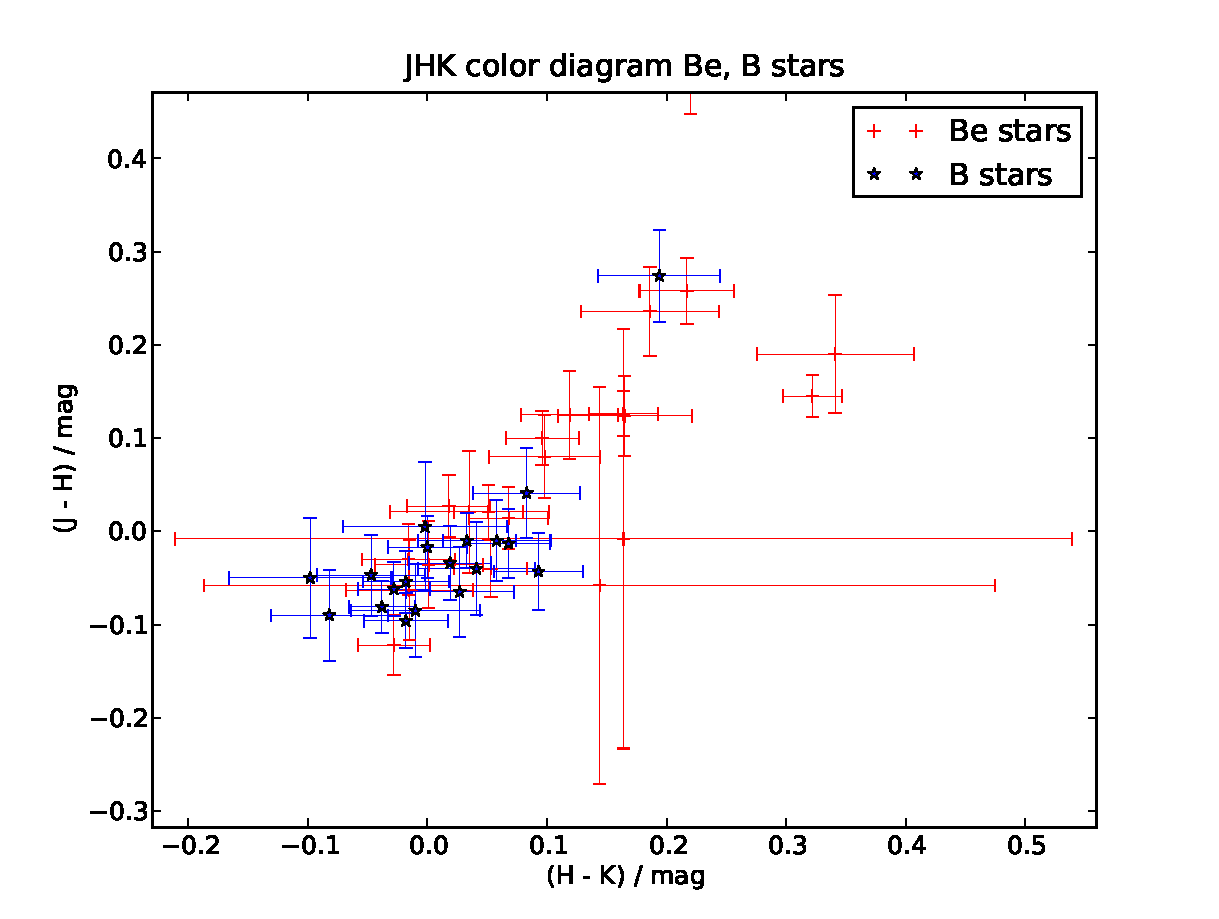
\includegraphics[scale =.6]{jhk_be_b_errors}
        \else
        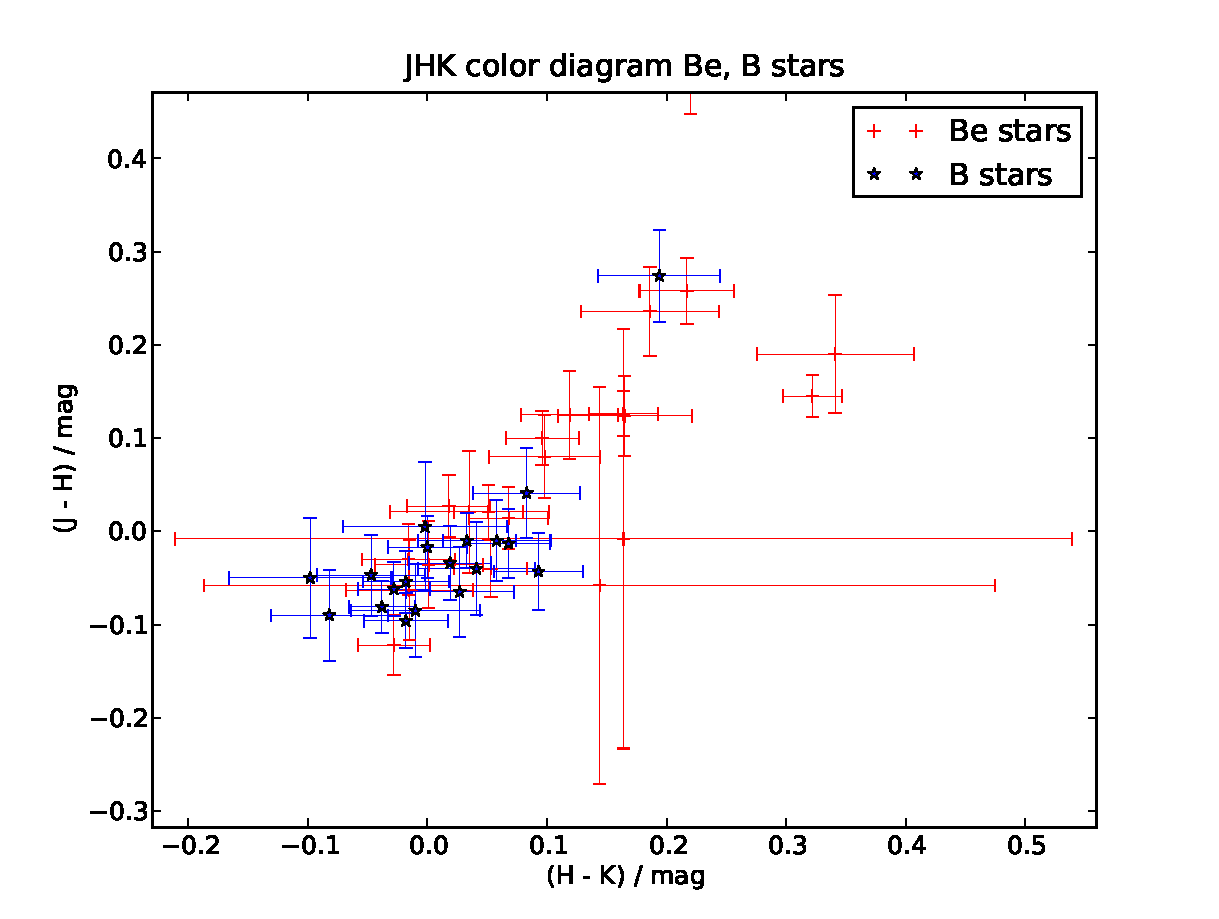
\includegraphics[bb = 92 86 545 742, height=6in]{jhk_be_b_errors}
        \fi
        \caption{Color diagram of confirmed Be stars Vs B stars with errors}
        \label{Figjhk_be_b_errors}
      \end{center}
    \end{figure}

\clearpage


\subsection{Classification}
Data were transformed from original VOTable obtained from Virtual
Observatory tools to arff\footnote{Attribute-Relation File
  Format. Developed by the Machine Learning Project at the Department
  of Computer Science of The University of Waikato.}format used in
Weka Data Mining system. Algorithm C4.5 (J48) was used to perform
actual classification with following result:

\begin{lstlisting}
  Correctly Classified Instances         769               73.0989 %
  Incorrectly Classified Instances       283               26.9011 %
  Kappa statistic                          0.4496
  Mean absolute error                      0.3843
  Root mean squared error                  0.4383
  Relative absolute error                 79.4985 %
  Root relative squared error             89.1648 %
  Total Number of Instances             1052
\end{lstlisting}

As seen on the first row 73 \% from  1052 objects were classified
correctly. More details can be obtained from confusion matrix below.

\begin{lstlisting}
  B   Be   <-- classified as
 304 126 |   B
 157 465 |   Be
\end{lstlisting}

304 of B and 456 of Be stars were classified correctly but 126 of B
and 157 of Be stars were classified incorrectly. In virtue of these
results one should be sceptical if the distinction based only on
photometric properties is significant enough to find relevant new
candidates of Be stars. For this reason more sophisticated (and much
more complicated) approach using spectra analysis was tested.

\section{Spectral Data Mining}
Spectra provide much wider scientific informations over photometric
properties. Spectral lines exibits many distingues features and
astronomers have long tradition of analysing their properties. On the
other side its much complicated ot handle them because of different
characteristics (resolution, calibration, wavelength range, etc). This
is especially true for massive automated processing.  

\subsection{Testing Data}
As testing sample the project SEGUE of SDSS were selected. This
contains 178315 spectra in DR7. Following SQL query was used to
generate the list of URL links for individual FITS files. These files
were then download to local sever using wget command.

\begin{lstlisting}
SELECT  objid,dbo.fGetUrlFitsSpectrum(s.specObjID)                                                           
INTO mydb.segue_1                                                                                     
FROM SpecPhotoAll s, platex p                                                                         
WHERE s.specObjID is not null                                                                         
AND s.plateid = p.plateid                                                                             
AND p.programname LIKE 'segue%'                                                                       
AND specClass = 1
\end{lstlisting}

\subsection{Training Data}
The spectra from Ondřejov Observatory were used as training
sample. Files were downloaded using SSA protocol. The SSA server is
not publically aviable, therefore SSH tunneling was used. Two scripts
for this process were created. First to construct the list of SSA
compliant adresses, the second to analyse acquired response in VOTable
format. Then the spectra were downloaded using wget command. The
fuction for constructing the links based on list of the RA, DEC which
were obtained from Hipparcos catalog using the specification of IDs
from Ondřejov's index.

\begin{lstlisting}
def createQuery(data):
    """ From raw data construct ra, dec """
    """ Convert to degrees """
    for line in data:
        ra = ac.AngularCoordinate(line[0:10]).degrees # convert ra to degrees
        dec = ac.AngularCoordinate(line[-13:-1]).degrees # convert dec to degrees
        ra = line[0]
        dec = line[1]
        ssaTemp = 'http://tvoserver/coude/coude.cgi?c=ssac&n=coude_ssa&REQUEST=queryData&POS=<ra>,<dec>&SIZE=1'
        ssaTemp = ssaTemp.replace('<ra>',"%0.3f" % ra)
        ssaTemp = ssaTemp.replace('<dec>',"%0.3f" % dec)
        ssa.append(ssaTemp)
    return ssa
\end{lstlisting}

The script generate the following output. The same process were used
later for obtaining th sample of non Be stars.

\begin{lstlisting}
http://tvoserver/coude/..._ssa&REQUEST=queryData&POS=83.113,-65.582&SIZE=60
http://tvoserver/coude/..._ssa&REQUEST=queryData&POS=162.537,148.333&SIZE=60
http://tvoserver/coude/..._ssa&REQUEST=queryData&POS=19.907,-73.502&SIZE=60
\end{lstlisting}


\subsubsection{Spectra Reduction}
Because spectra from SDSS and Ondřejov Observatory had different
resolution, reduction was needed. First the parameter CD1\_1 (Coordinate
increment per pixel) had to be obtained form FITS file.


\begin{lstlisting}
  In [1]: hdu = pf.open('sdss_test.fit')
  In [2]: hdu[0].header['CD1_1']
  Out[2]: 0.0001 # SDSS spectrum 
  Out[3]: 0.2567 # Onřejov spectrum
\end{lstlisting}

Spectra in SDSS are stored in logarithmic scale thus the value is
computed as $ 10^{CD1\_1} = 1.00$. The ratio is then
$CD1\_1_{SDSS}/CD1\_1_{OND} = 3.87$. Based on this computation 4
pixels of Ondřejov's spectra were reduced into one. There is the
critical part of the reduction program:

\begin{lstlisting}
 def convolution(f, g):
    """ Convolve two functions"""
    fg = np.convolve(g,f,'same')
    return fg
 def reduce(x,y,bin):
    """ Reduce bin pixel into 1"""
    size = x.size/bin
    l = 0
    xx = x[:x.size-1:bin]
    yy = list()
    for i in range(0,size):
        s = 0
        for j in range(0,bin):
            s = s + y[l]
            l+=1
        yy.append(s/bin)
    return xx, yy
\end{lstlisting}

Prior to binning pixels convolution with gaussian function was
performed on the spectra. Convolution is defined:

\begin{equation}
  \label{eq:convolution}
 (f * g )(t) \stackrel{\mathrm{def}}{=}\ \int_{-\infty}^{\infty} f(\tau)\, g(t - \tau)\, d\tau
\end{equation}
 
Here it was used in it's dicrete form

\begin{equation}
  \label{eq:discreteConvolution}
  (f * g)[n]\ \stackrel{\mathrm{def}}{=}\ \sum_{m=-\infty}^{\infty} f[m]\, g[n - m]
\end{equation}



The result is on the figure


    \begin{figure}[!htbp]
      \begin{center}
        \leavevmode
        \ifpdf
        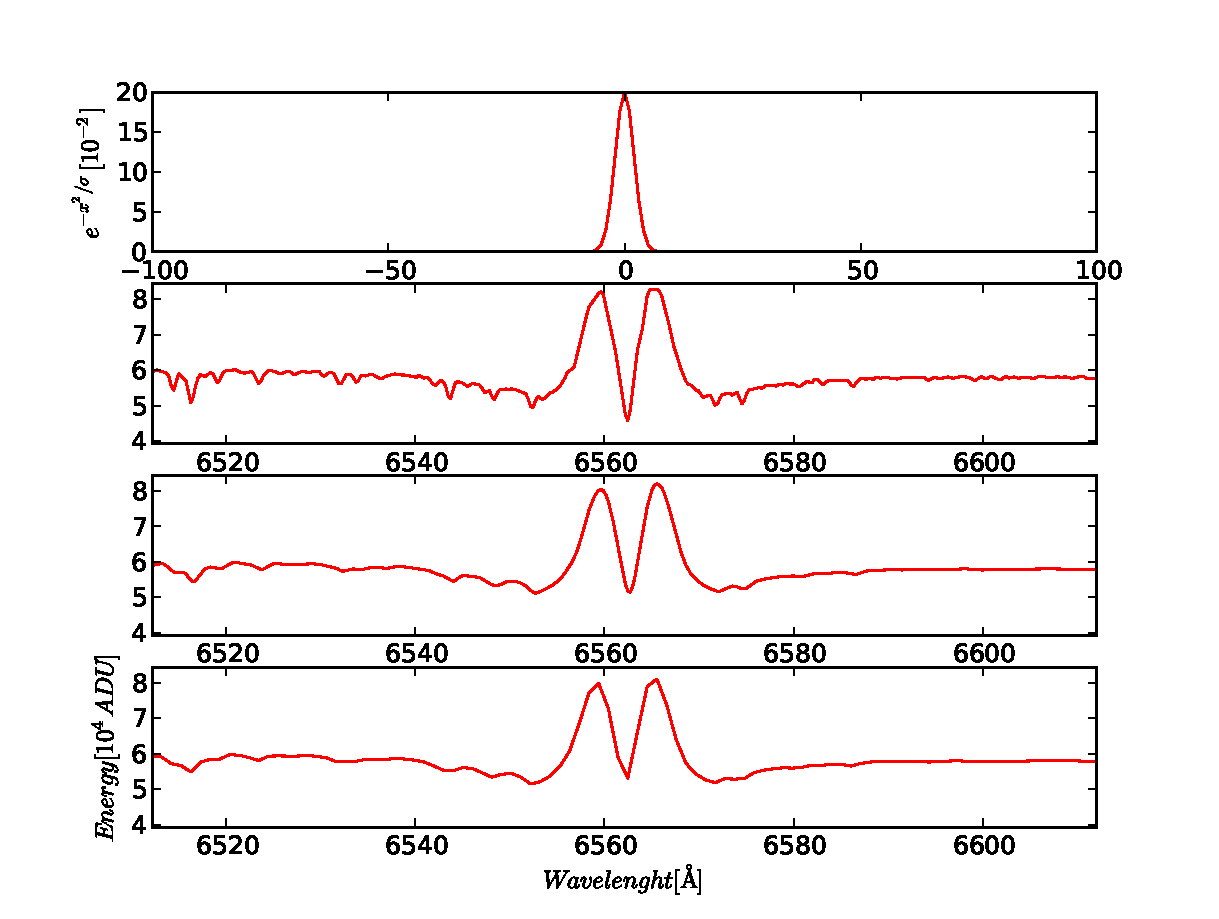
\includegraphics[scale =.8]{convolution}
        \else
        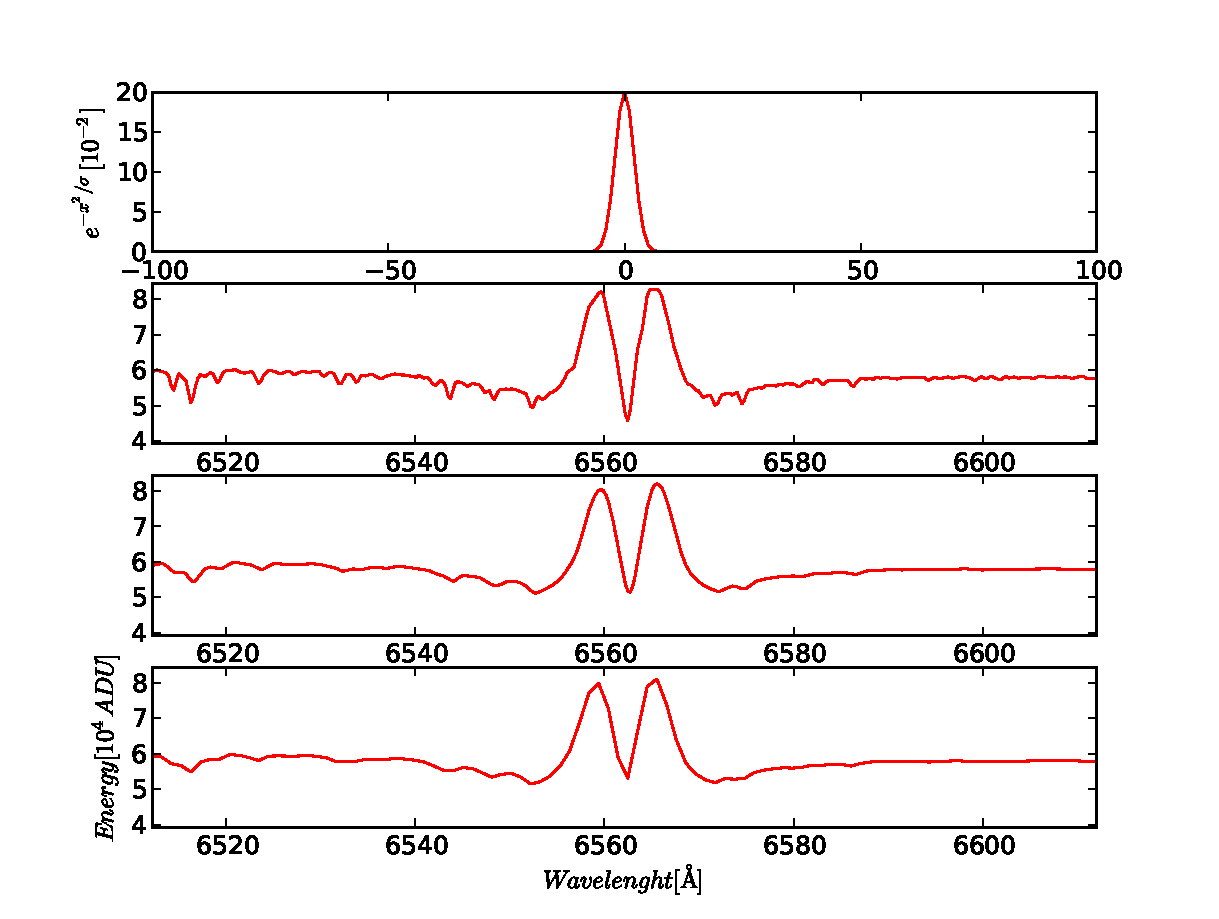
\includegraphics[bb = 92 86 545 742, height=6in]{convolution}
        \fi
        \caption{Reduction of Ondřejov's spectra of the Be star 4
          Hercules. The top figure shows gaussian function used for
          convolution with the structrum, followed by the original
          spectrum then there is a spectrum after convolution with the
          gausian function. The last is the final spectrum after
          reduction.}
        \label{FigReduction}
      \end{center}
    \end{figure}

\clearpage




\subsection{Spectra Lines Characteristics}
As parameters for Data Mining process characteristics value of
H$\alpha$ line were extracted from the spectra. Many possible
characteristics from fitting functions through Wavelets Coefficients
and Eigen Values were discussed with experts. Three parameters were
finally slected. The hight and the width of the H$\alpha$ emission
line and median absolute deviation as a characterization of the noise
level in the spectrum. 


\subsubsection{Normalization}
Spectra from SDSS are normalized but the spectra from Ondřejov are
not. The spectra were devided by it's continuum fit function. This
process ensures the compatibility when comparing different
spectra. Function polyfit from numpy package was used to perfom the
fit. The solution minimizes the squared error:

\begin{align}
  \frac{d}{dq} \sum_{i = 1}^n{(y_i - \operatorname{f}(x_i) )^2} = 0,
\end{align}

where $\operatorname{f}$ is in our case $\operatorname{f}(x) = q_1x +
q_0$.

\subsubsection{The hight of the H$\alpha$ line}
The maximum value in the region of $50\AA$ were extracted from the
spectrum.

\begin{lstlisting}
def getMax(x,y,line,range):
    """ Return maximum value of range in the spectrum"""
    xrange = x[(x < line + range) & (x > line - range)]
    yrange = y[(x < line + range) & (x > line - range)] - 1
    maximum = yrange.max()
    minimum = yrange.min()
    if abs(maximum)  > abs(minimum):
        extrem =  maximum 
    else:
        extrem = minimum 
    return xrange, extrem, sgn
\end{lstlisting}

\subsubsection{The noise level of the spectrum}
The noise in the spectrum contributes to the characteristics of the
spectral lines. As ans estimetor of the noise level the median
absolute deviation was used. It is defined as:

\begin{align}
  \operatorname{mad} = \operatorname{median}_{i}\left(\ \left| X_{i} -
      \operatorname{median}_{j} (X_{j}) \right|\ \right)
\end{align}

\subsubsection{The width of the H$\alpha$ line}
The gaussian function was fitted to the spectral line. First the
robust estimators were computed and used as input parameters for
leastsq\footnote{"leastsqi"s a wrapper around MINPACK’s lmdif and
  lmder algorithms.} method from scipy.opt module, which minimize the
sum of squares.

\begin{align}
  x_0 & = \frac{\operatorname{median}(w_jx_j)}{\sum{w_i}}, \\
  S & = \frac{\operatorname{mad}(x_i - x_0)}{\sum{w_i}}.
\end{align}

Part of the script implementing fitting the gaussian function

\begin{lstlisting}
x0 = np.median(sum(w*x))/sum(w)
S = sum(w*mad((x - x0)))/sum(w)
params = np.array([1, maximum, x0, S], dtype=float)
fit, flag = opt.leastsq(residuals, params, args=(yrange, xrange))
gauss = model(xrange, fit) + 1

def model(t, coeffs):
    return coeffs[0] + coeffs[1] * np.exp( - ((t-coeffs[2])/coeffs[3])**2 )
def residuals(coeffs, y, t):
    return y - model(t, coeffs)
\end{lstlisting}

The final result is on the figure \ref{FigSpecChar1} and
\ref{FigSpecChar2}. The script was adjust to work with SDSS and
Ondřejov's spectra. The whole procedure was performed on all of the
cca 200 000 SDSS spectra and few dozens Ondřejov's spectra resulting
with the ASCII files with the characteristic values used later in Data
Mining process.

   \begin{figure}[!htbp]
      \begin{center}
        \leavevmode
        \ifpdf
        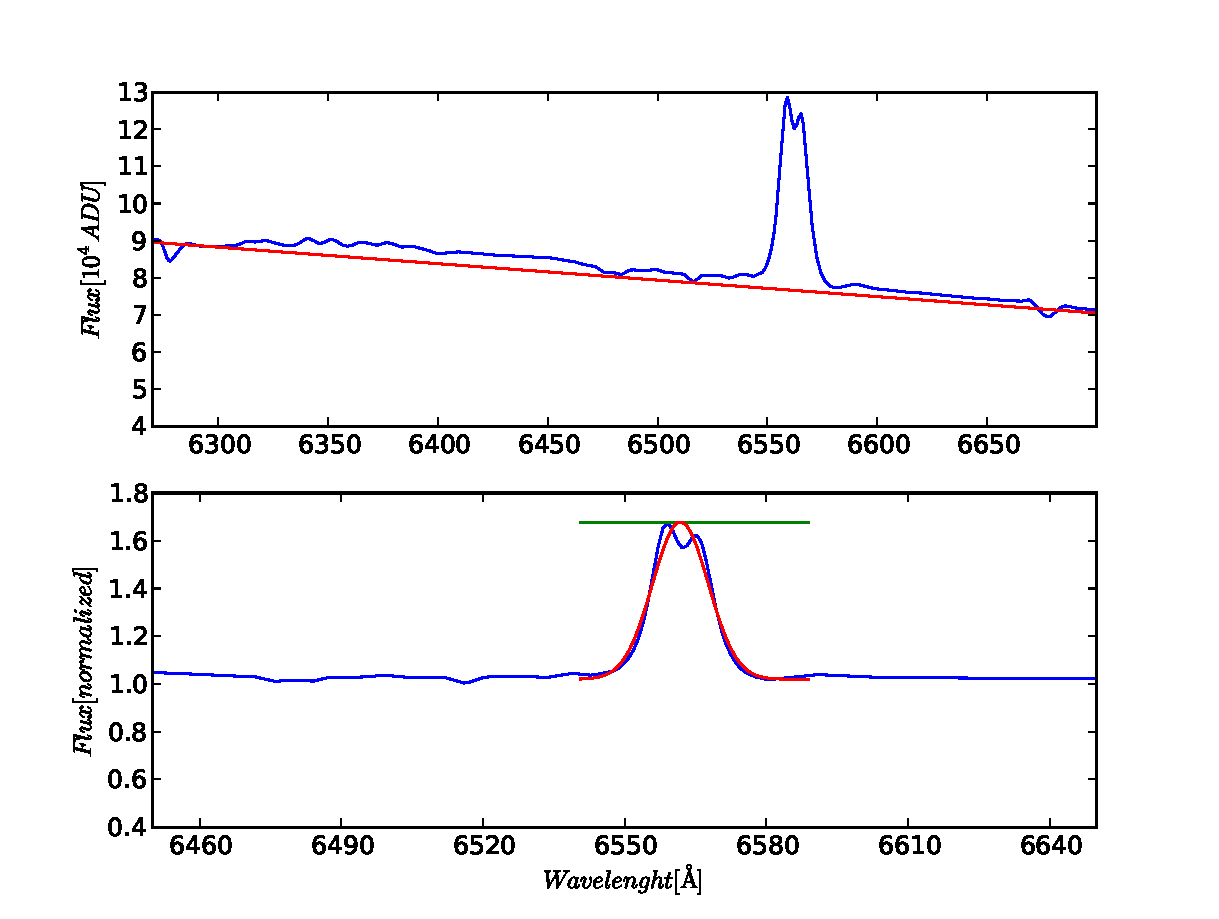
\includegraphics[scale =.8]{figSpecCharCyg60}
        \else
        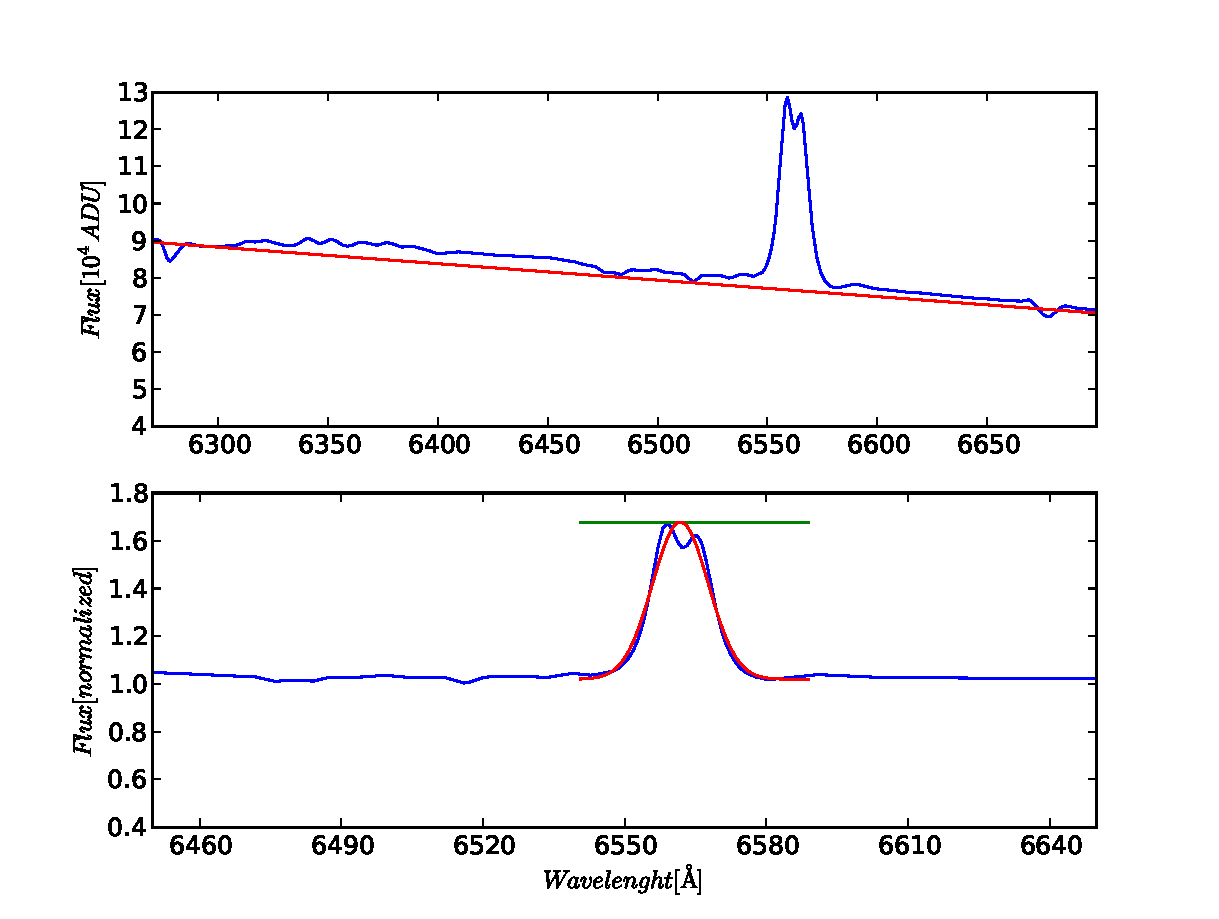
\includegraphics[bb = 92 86 545 742, height=6in]{figSpecCharCyg60}
        \fi
        \caption{Normalized spectrum of Be star 60 Cyg. The top figure
          depicts the continuum fit. The bottom figure shows the
          region (width of the green line) used for extraction. The
          position of the line correspond to the maximum value in the
          region of $50\AA$. The gaussian fit is in red.}
        \label{FigSpecChar}
      \end{center}
    \end{figure}

   \begin{figure}[!htbp]
      \begin{center}
        \leavevmode
        \ifpdf
        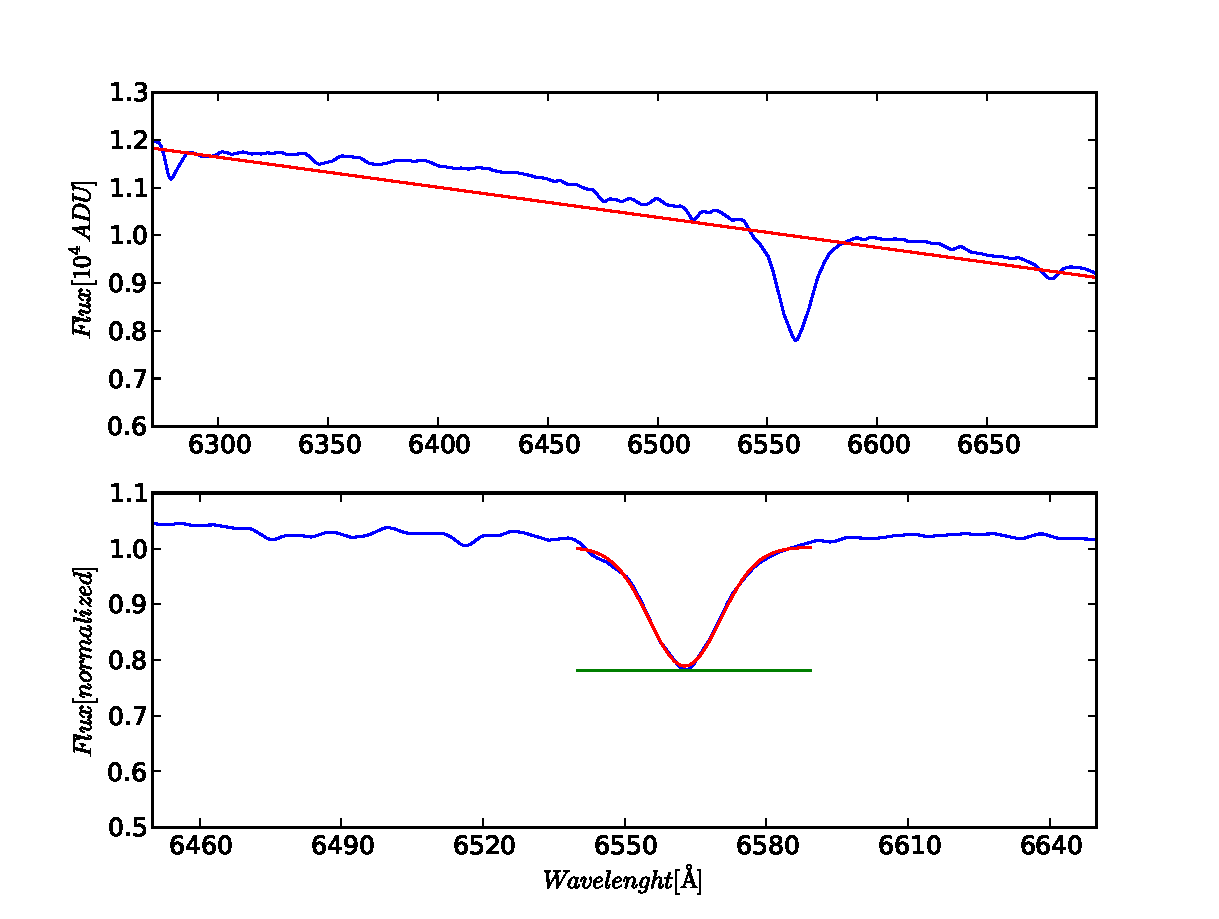
\includegraphics[scale =.8]{figSpecCharhd216057}
        \else
        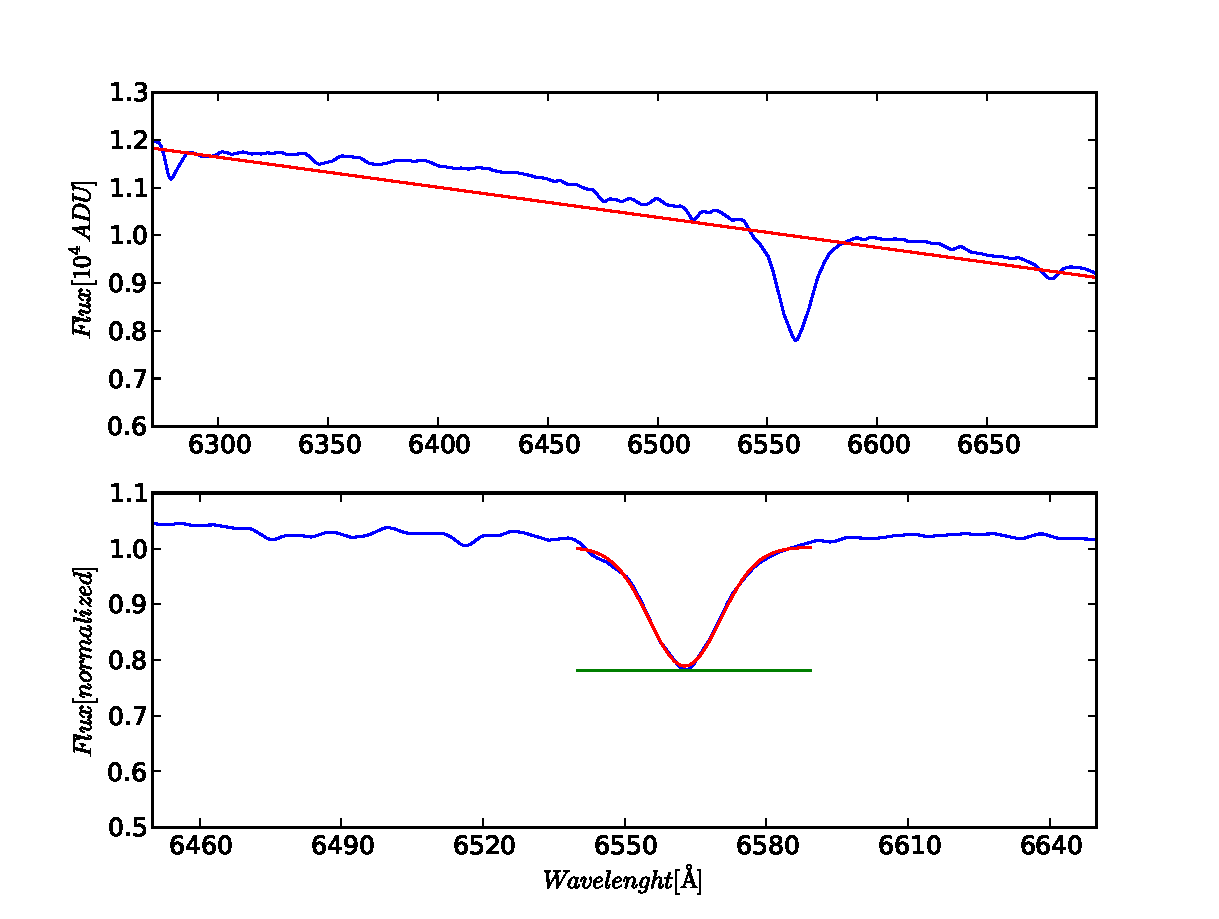
\includegraphics[bb = 92 86 545 742, height=6in]{figSpecCharhd216057}
        \fi
        \caption{Normalized spectrum of Be star HR 8682. The top
          figure depicts the continuum fit. The bottom figure shows
          the region (width of the green line) used for
          extraction. The position of the line correspond to the
          maximum value in the region of $50\AA$. The gaussian fit is
          in red.}
        \label{FigSpecChar}
      \end{center}
    \end{figure}


\clearpage

% The script was written to normalize the spectrum and extract the line
% characteristic value. This program also plots the results of the
% process as it is shown on previous picture. The function used to
% extract the line characteristic value is below.



\subsection{Data Mining}
Classification was performed using weka software with algoritm J48
described in the chapter \ref{chap:dataMining}. Trainning set had 183
and testing set 178314 items. The excerpt from these files follows.

\begin{lstlisting}
@RELATION STAR-B-BE
@ATTRIBUTE name STRING
@ATTRIBUTE alpha NUMERIC
@ATTRIBUTE grp {be,o}
@DATA
10_cas,-0.822196556626,be
11_cyg,1.68689566629,be
\end{lstlisting}

\begin{lstlisting}
@RELATION STAR-B-BE
@ATTRIBUTE name STRING
@ATTRIBUTE alpha NUMERIC
@ATTRIBUTE grp {be,o}
@DATA	 
spSpec-53228-1884-001	-0.584628294569	 ?
spSpec-53228-1884-002	-0.877184482566	 ?
\end{lstlisting}

The attribute \textrm{grp} is known for the trainnig set but uknown
for testing set. The classification process fills this information
based on decision tree created during learning phase. To automte the
process command line verson of weka software was used.

\begin{lstlisting}
  java -classpath weka.jar
  weka.classifiers.meta.FilteredClassifier -F
  weka.filters.unsupervised.attribute.RemoveType -W
  weka.classifiers.trees.J48 -t $1 -T $2 -p 1
\end{lstlisting}


\subsection{Results}

Because only one parameter (H$\alpha$) was used, the decision tree is
very simple. If the value of the parametr is greater than $-0.464633$
the object is considered to be a Be star. If the values in the range
of $-0.676474$ and $-0.464633$ it is considered to be non Be star (no
further restriction was assert on the \textrm{other} group). It imply
that according to classifier the Be star is an object with extreme
values in H$\alpha$ line. This outcome does not oppose our
undestanding of these kind of objects.


\begin{lstlisting}
  J48 pruned tree
------------------
alpha <= -0.464633
|   alpha <= -0.676474: be (45.0/18.0)
|   alpha > -0.676474: o (46.0/5.0)
alpha > -0.464633: be (92.0/16.0)
\end{lstlisting}

\begin{lstlisting}
  === Summary ===
Correctly Classified Instances         142               77.5956 %
Incorrectly Classified Instances        41               22.4044 %
Kappa statistic                          0.5078
Mean absolute error                      0.3215
Root mean squared error                  0.4083
Relative absolute error                 66.4104 %
Root relative squared error             83.0045 %
Total Number of Instances              183     
\end{lstlisting}

\begin{lstlisting}
  === Confusion Matrix ===
 Be     O   <-- classified as
 102    6 |   Be
  35   40 |   Othres
\end{lstlisting}

Confusion Matrix indicates that the classifier is much better in
predicting Be stars (102/6 correct assigments) then in predicting
results in the \textrm{others} group where there are just 40/35 right
assigments.

Spectra of some of the objects classified as Be stars are presented
here. 


   \begin{figure}[!htbp]
      \begin{center}
        \leavevmode
        \ifpdf
        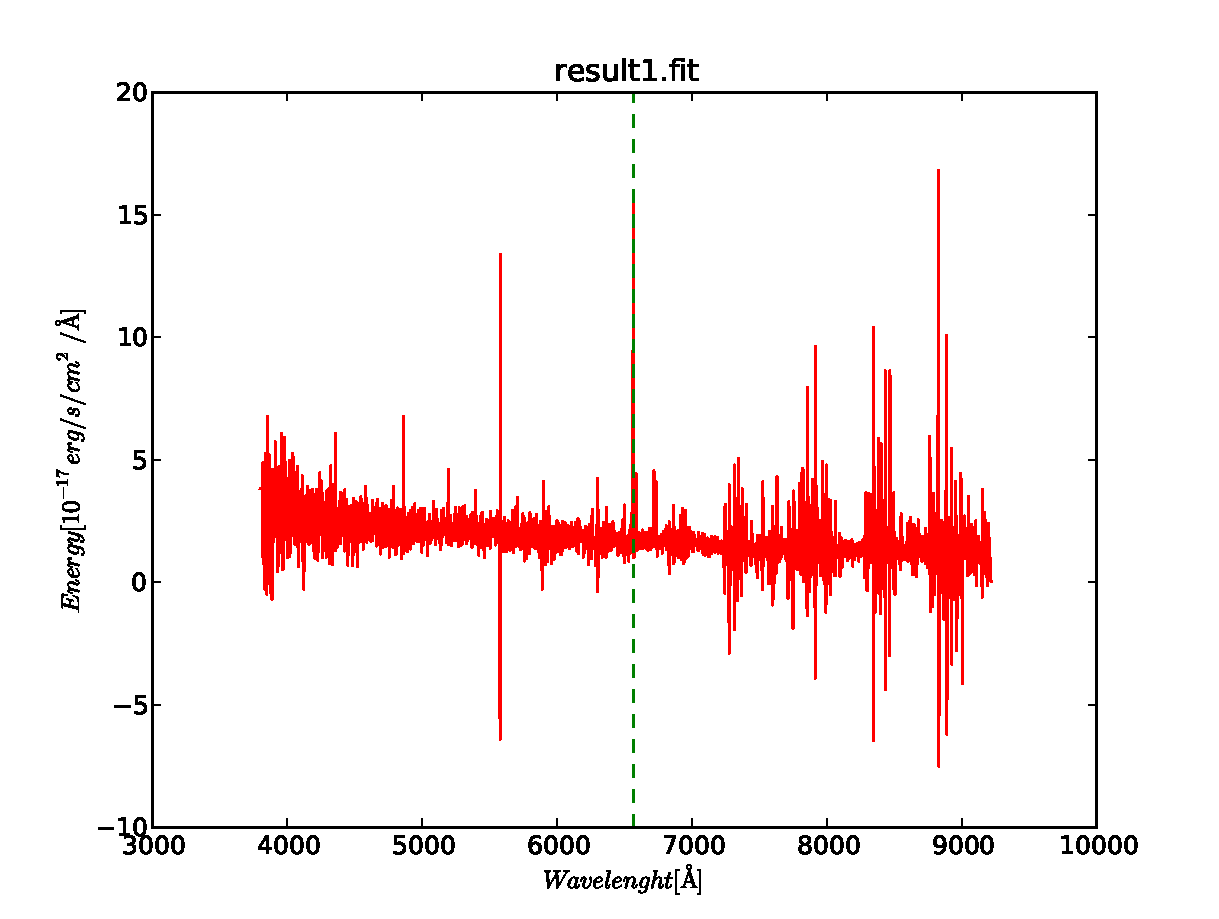
\includegraphics[scale =.8]{result1}
        \else
        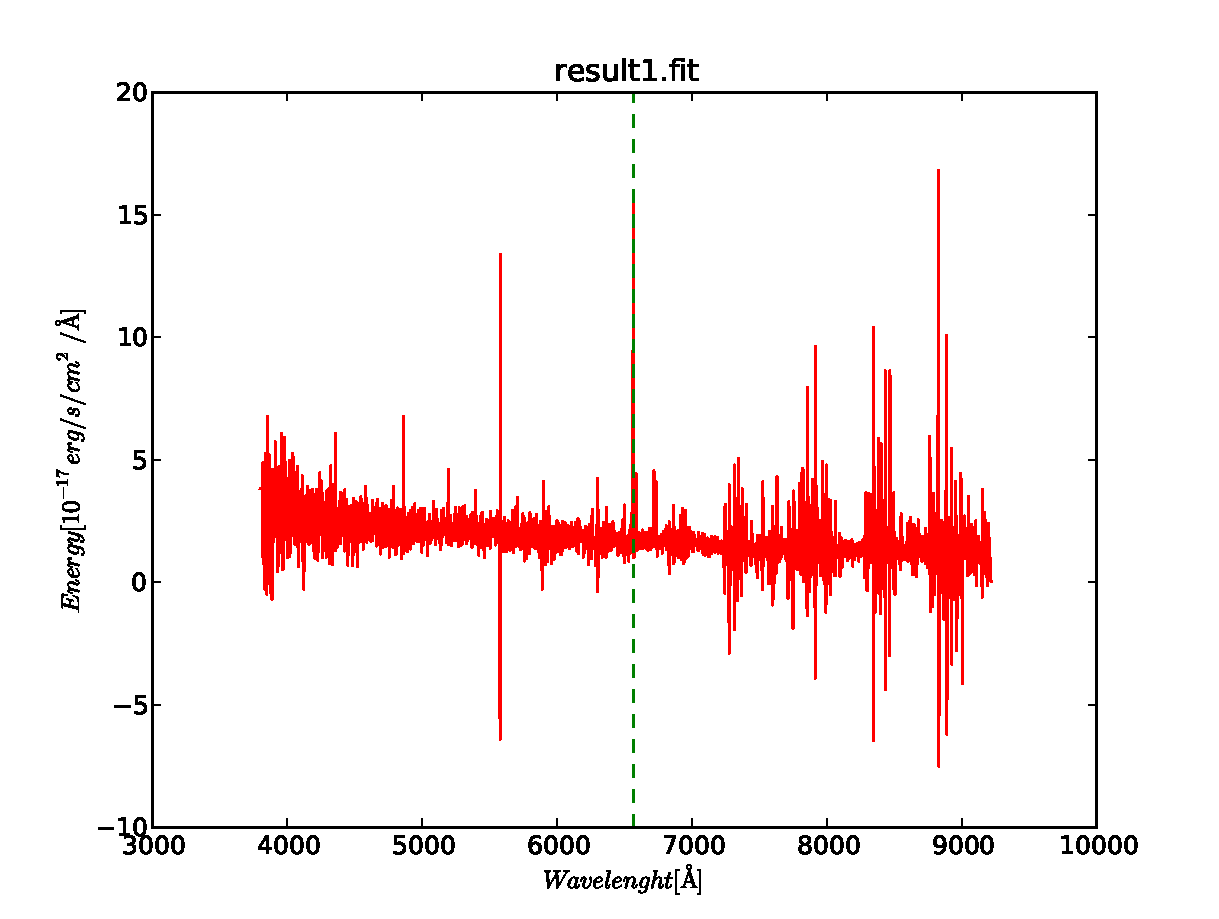
\includegraphics[bb = 92 86 545 742, height=6in]{result1}
        \fi
        \caption{Spectrum of }
        \label{FigResult1}
      \end{center}
    \end{figure}

   \begin{figure}[!htbp]
      \begin{center}
        \leavevmode
        \ifpdf
        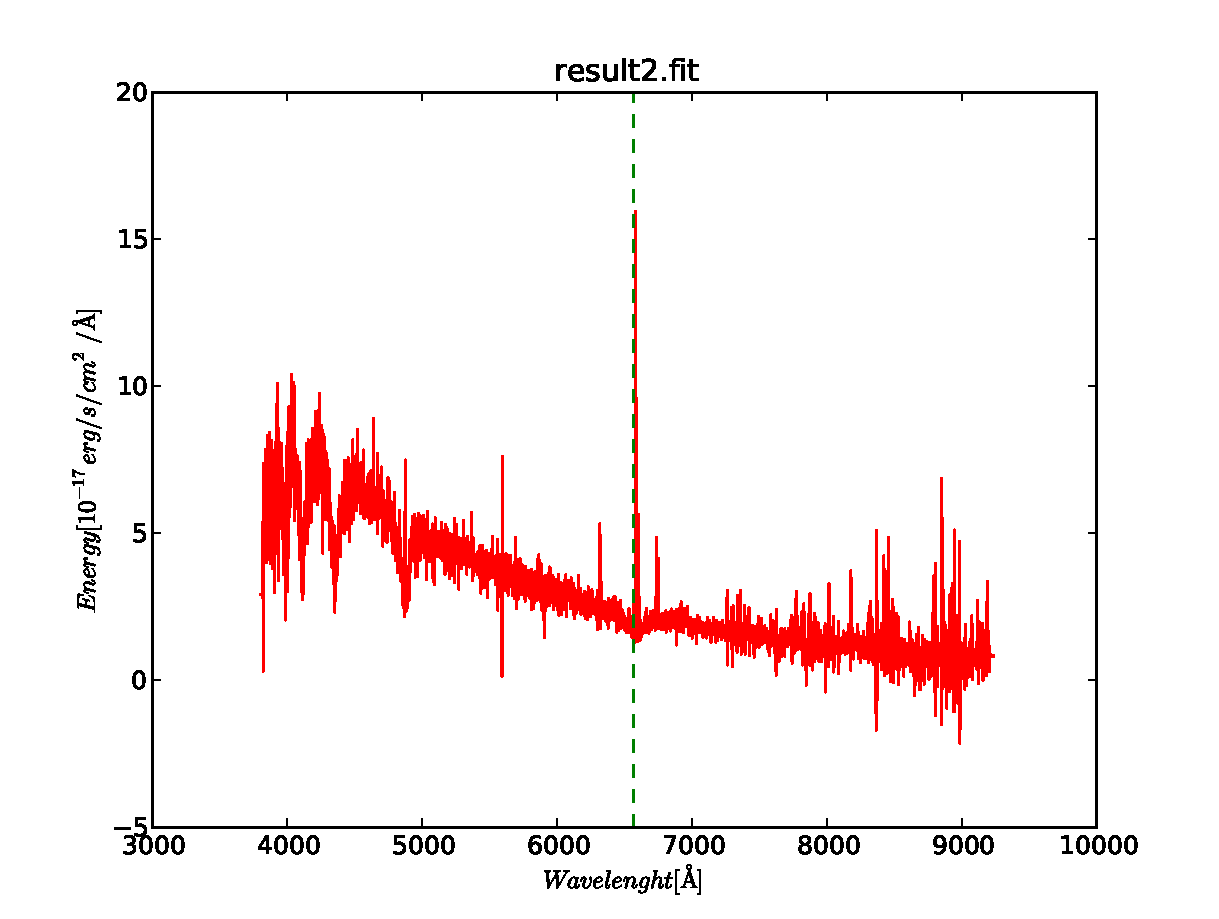
\includegraphics[scale =.8]{result2}
        \else
        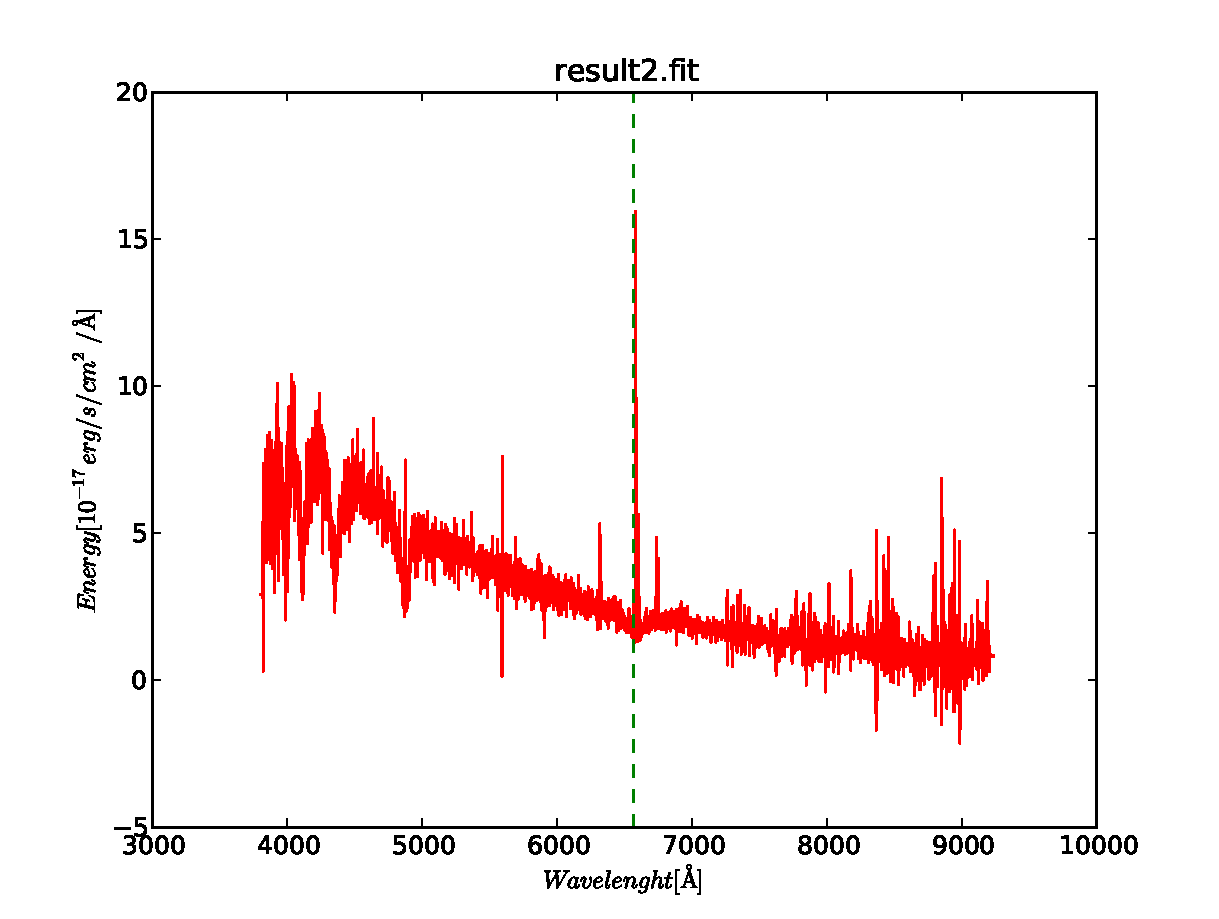
\includegraphics[bb = 92 86 545 742, height=6in]{result2}
        \fi
        \caption{Spectrum of }
        \label{FigResult2}
      \end{center}
    \end{figure}

   \begin{figure}[!htbp]
      \begin{center}
        \leavevmode
        \ifpdf
        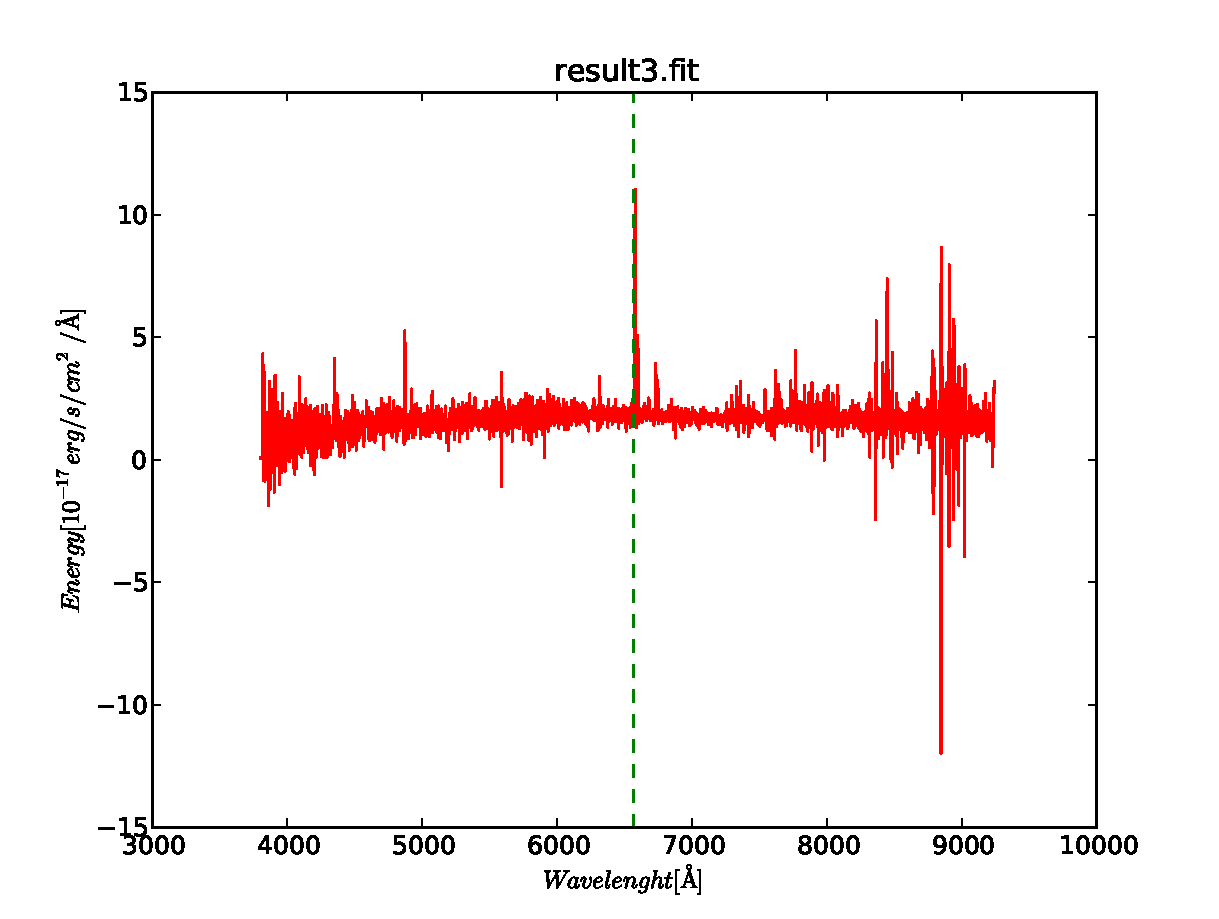
\includegraphics[scale =.8]{result3}
        \else
        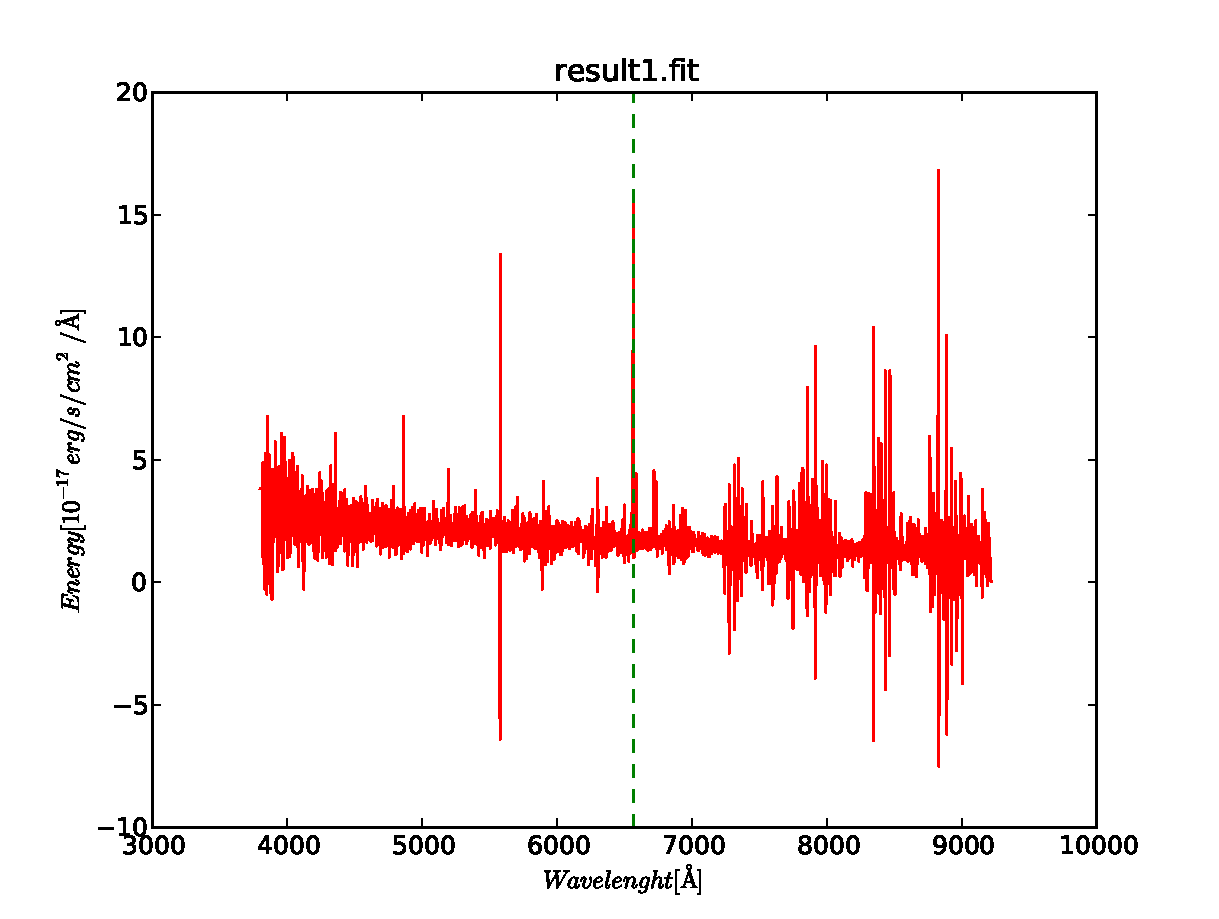
\includegraphics[bb = 92 86 545 742, height=6in]{result1}
        \fi
        \caption{Spectrum of }
        \label{FigResult3}
      \end{center}
    \end{figure}

% Samples of Be Stars           
 
    For comparison there are spectra of know Be stars. It is clear
    that the profile of the H$\alpha$ line is complex and just one
    parameter cannot possibly express it's characteristic. More
    advaced description such as Wavelets coeffiction or theoretical
    models of the line is needed if we want to create realiable
    process for indentifying Be stars.

   \begin{figure}[!htbp]
      \begin{center}
        \leavevmode
        \ifpdf
        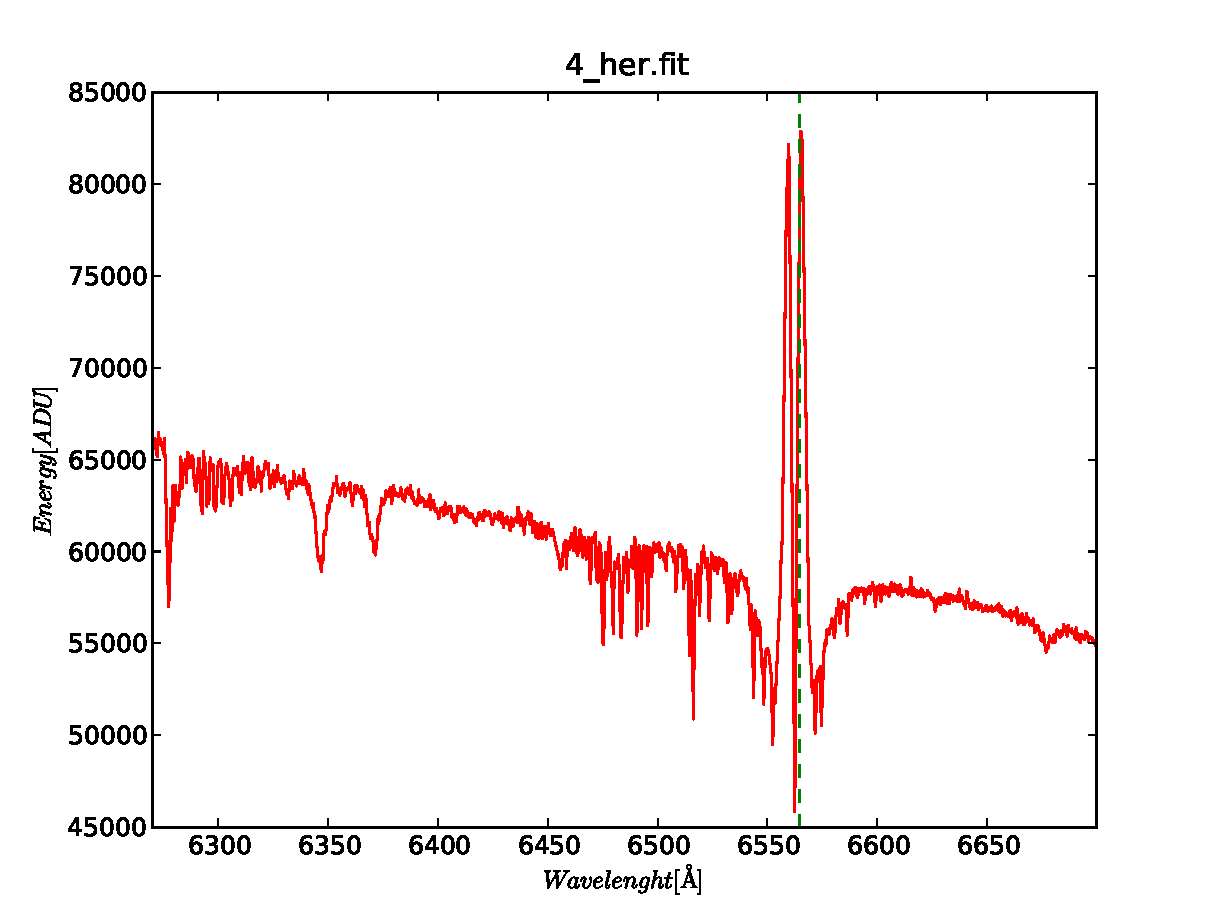
\includegraphics[scale =.8]{be1_4_her}
        \else
        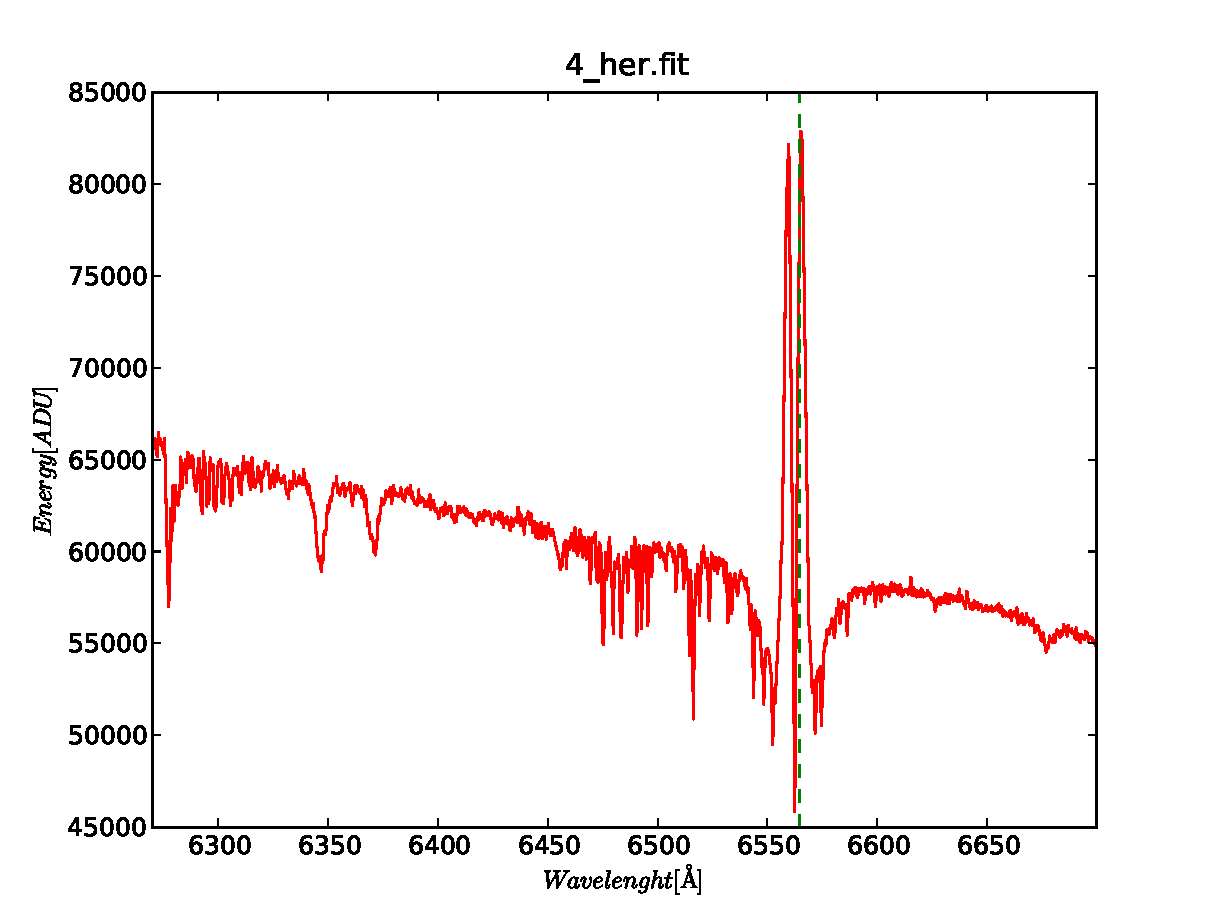
\includegraphics[bb = 92 86 545 742, height=6in]{be1_4_her}
        \fi
        \caption{Spectrum of 4 Her. Be star. Spectral Type B9pe.  }
        \label{FigBe1}
      \end{center}
    \end{figure}

   \begin{figure}[!htbp]
      \begin{center}
        \leavevmode
        \ifpdf
        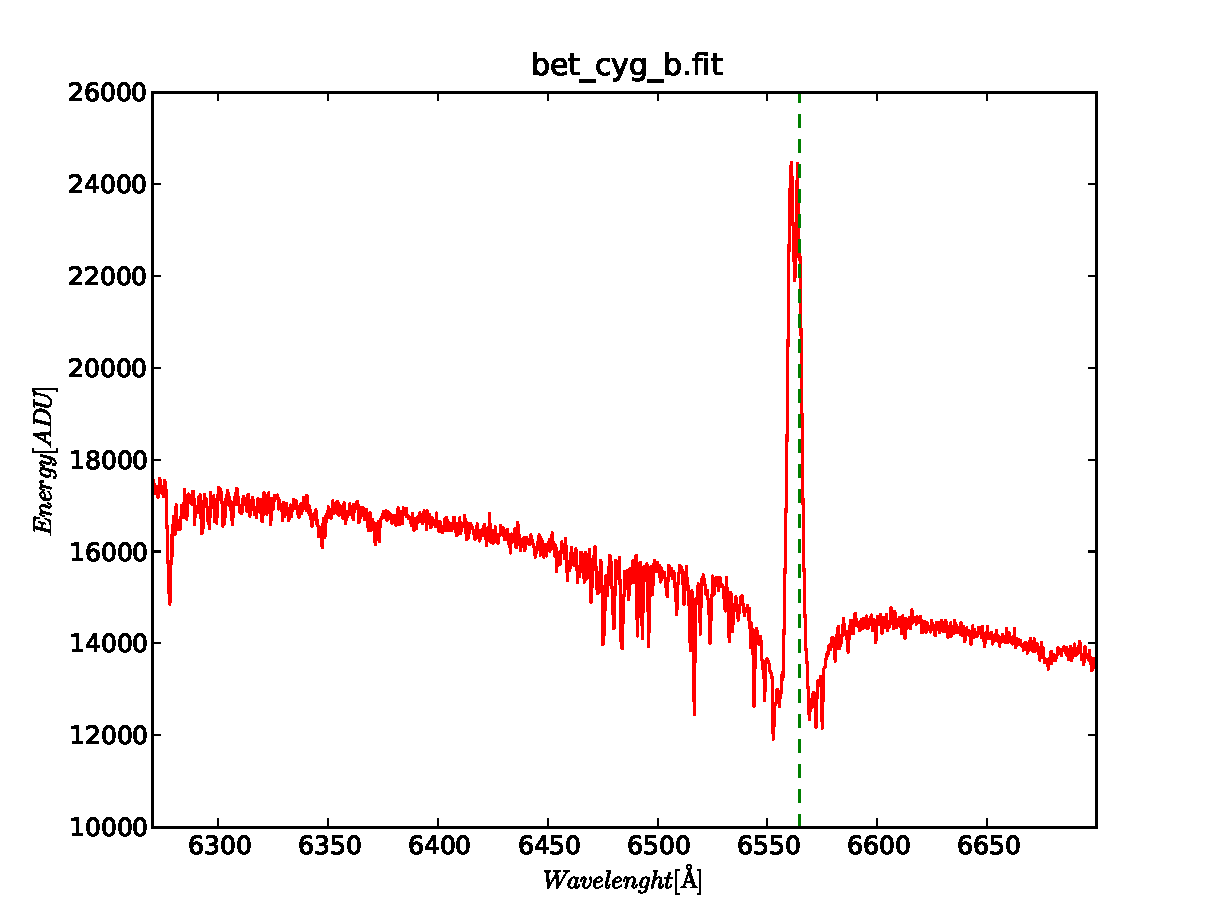
\includegraphics[scale =.8]{be4_bet_cyg_b}
        \else
        \includegraphics[bb = 92 86 545 742, height=6in]{be4_bet_cyg_b}
        \fi
        \caption{Spectrum of HR 7418 (Albireo B). A fast-rotating Be
          star, with an equatorial rotational velocity of at least 250
          kilometers per second. Its surface temperature has been
          spectroscopically estimated to be about 13.200 K. Spectral
          Type B8Ve. }
        \label{FigBe4}
      \end{center}
    \end{figure}

   \begin{figure}[!htbp]
      \begin{center}
        \leavevmode
        \ifpdf
        \includegraphics[scale =.8]{be3_6_cep}
        \else
        \includegraphics[bb = 92 86 545 742, height=6in]{be3_6_cep}
        \fi
        \caption{Spectrum of 6 Cepheus. Be star. Spectral Type B3IVe.}
        \label{FigBe3}
      \end{center}
    \end{figure}



\clearpage


\subsection{Conclusion}

The harvesting of large-scale of spectral data is challenging but
solvable problem. The technology of Virual Observatory offers solid
background for data discovery and retrieval. The whole process can be
automated using UN*X like approach of small and single purpose scripts
or programs. The last stage of choosing the right characteristics and
Data Mining method is even more complex task requiring deep
understanding of the researched phenomenas and Machine Learnig theory
and technology. The possible solution can be based on cooperation
between experts in scientific and computer science field. Without such
collaboration we are missing lots of opportunities.



% mad2
=== Run information ===

Scheme:       weka.classifiers.trees.J48 -C 0.25 -M 2
Relation:     STAR-BE-O-weka.filters.unsupervised.attribute.Remove-R1
Instances:    173
Attributes:   4
              max
              width
              mad
              grp
Test mode:    10-fold cross-validation

=== Classifier model (full training set) ===

J48 pruned tree
------------------

max <= -0.18843
|   max <= -0.324763: o (46.0/5.0)
|   max > -0.324763
|   |   max <= -0.255475
|   |   |   mad <= 0.004133: o (2.0)
|   |   |   mad > 0.004133: be (13.0/1.0)
|   |   max > -0.255475
|   |   |   mad <= 0.009862: o (10.0)
|   |   |   mad > 0.009862
|   |   |   |   width <= 7.621593: o (3.0/1.0)
|   |   |   |   width > 7.621593: be (2.0)
max > -0.18843
|   mad <= 0.030316
|   |   max <= -0.091726
|   |   |   width <= 5.286489
|   |   |   |   max <= -0.170022: be (2.0)
|   |   |   |   max > -0.170022: o (3.0)
|   |   |   width > 5.286489: be (9.0)
|   |   max > -0.091726: be (76.0)
|   mad > 0.030316
|   |   max <= 6.917615: o (4.0)
|   |   max > 6.917615: be (3.0)

Number of Leaves  : 	12

Size of the tree : 	23


Time taken to build model: 0.12 seconds

=== Stratified cross-validation ===
=== Summary ===

Correctly Classified Instances         145               83.815  %
Incorrectly Classified Instances        28               16.185  %
Kappa statistic                          0.6529
Mean absolute error                      0.1849
Root mean squared error                  0.3652
Relative absolute error                 39.8819 %
Root relative squared error             75.8919 %
Total Number of Instances              173     

=== Detailed Accuracy By Class ===

               TP Rate   FP Rate   Precision   Recall  F-Measure   ROC Area  Class
                 0.864     0.206      0.88      0.864     0.872      0.882    be
                 0.794     0.136      0.769     0.794     0.781      0.882    o
Weighted Avg.    0.838     0.181      0.839     0.838     0.839      0.882

=== Confusion Matrix ===

  a  b   <-- classified as
 95 15 |  a = be
 13 50 |  b = o

%\def\baselinestretch{1}
\chapter{My Conclusions ...}
\ifpdf
    \graphicspath{{Conclusions/ConclusionsFigs/PNG/}{Conclusions/ConclusionsFigs/PDF/}{Conclusions/ConclusionsFigs/}}
\else
    \graphicspath{{Conclusions/ConclusionsFigs/EPS/}{Conclusions/ConclusionsFigs/}}
\fi

\def\baselinestretch{1.66}

Here I put my conclusions ...

%%% ----------------------------------------------------------------------

% ------------------------------------------------------------------------

%%% Local Variables: 
%%% mode: latex
%%% TeX-master: "../thesis"
%%% End: 


\backmatter % book mode only
\appendix
%\graphicspath{{pic/results/}}
\chapter{Appendix1: Spectra of Be candidates}
List of 46 objects from SDSS obtained by data mining process described
in section \ref{sec:spectral}.

\centerline{
\begin{tabular}{cc}
  \includegraphics[width=0.50\textwidth]{1} &
  \includegraphics[width=0.50\textwidth]{2} \\
  \includegraphics[width=0.50\textwidth]{3} &
  \includegraphics[width=0.50\textwidth]{4} \\
  \includegraphics[width=0.50\textwidth]{5} &
  \includegraphics[width=0.50\textwidth]{6}
  \end{tabular}
}
\centerline{
\begin{tabular}{cc}
  \includegraphics[width=0.50\textwidth]{7} &
  \includegraphics[width=0.50\textwidth]{8} \\
  \includegraphics[width=0.50\textwidth]{9} &
  \includegraphics[width=0.50\textwidth]{10} \\
  \includegraphics[width=0.50\textwidth]{11} &
  \includegraphics[width=0.50\textwidth]{12} \\
  \includegraphics[width=0.50\textwidth]{13} &
  \includegraphics[width=0.50\textwidth]{14} 
  \end{tabular}
}

\centerline{
\begin{tabular}{cc}
  \includegraphics[width=0.50\textwidth]{15} &
  \includegraphics[width=0.50\textwidth]{16} \\
  \includegraphics[width=0.50\textwidth]{17} &
  \includegraphics[width=0.50\textwidth]{18} \\
  \includegraphics[width=0.50\textwidth]{19} &
  \includegraphics[width=0.50\textwidth]{20} \\
  \includegraphics[width=0.50\textwidth]{21} &
  \includegraphics[width=0.50\textwidth]{22} 
  \end{tabular}
}
\centerline{
\begin{tabular}{cc}
  \includegraphics[width=0.50\textwidth]{23} &
  \includegraphics[width=0.50\textwidth]{24} \\
  \includegraphics[width=0.50\textwidth]{25} &
  \includegraphics[width=0.50\textwidth]{26} \\
  \includegraphics[width=0.50\textwidth]{27} &
  \includegraphics[width=0.50\textwidth]{28} \\
  \includegraphics[width=0.50\textwidth]{29} &
  \includegraphics[width=0.50\textwidth]{30} 
  \end{tabular}
}
\centerline{
\begin{tabular}{cc}
  \includegraphics[width=0.50\textwidth]{31} &
  \includegraphics[width=0.50\textwidth]{32} \\
  \includegraphics[width=0.50\textwidth]{33} &
  \includegraphics[width=0.50\textwidth]{34} \\
  \includegraphics[width=0.50\textwidth]{35} &
  \includegraphics[width=0.50\textwidth]{36} \\
  \includegraphics[width=0.50\textwidth]{37} &
  \includegraphics[width=0.50\textwidth]{38} 
  \end{tabular}
}
\centerline{
\begin{tabular}{cc}
  \includegraphics[width=0.50\textwidth]{39} &
  \includegraphics[width=0.50\textwidth]{40} \\
  \includegraphics[width=0.50\textwidth]{41} &
  \includegraphics[width=0.50\textwidth]{42} \\
  \includegraphics[width=0.50\textwidth]{43} &
  \includegraphics[width=0.50\textwidth]{44} \\
  \includegraphics[width=0.50\textwidth]{45} &
  \includegraphics[width=0.50\textwidth]{46} 
  \end{tabular}
}

%\graphicspath{{pic/be/}}
\chapter{Appendix2: Spectra of Be stars from Ond\v rejov}
\centerline{
\begin{tabular}{cc}
  \includegraphics[width=0.50\textwidth]{1} &
  \includegraphics[width=0.50\textwidth]{2} \\
  \includegraphics[width=0.50\textwidth]{3} &
  \includegraphics[width=0.50\textwidth]{4} \\
  \includegraphics[width=0.50\textwidth]{5} &
  \includegraphics[width=0.50\textwidth]{6}
  \end{tabular}
}
\centerline{
\begin{tabular}{cc}
  \includegraphics[width=0.50\textwidth]{7} &
  \includegraphics[width=0.50\textwidth]{8} \\
  \includegraphics[width=0.50\textwidth]{9} &
  \includegraphics[width=0.50\textwidth]{10} \\
  \includegraphics[width=0.50\textwidth]{11} &
  \includegraphics[width=0.50\textwidth]{12} \\
  \includegraphics[width=0.50\textwidth]{13} &
  \includegraphics[width=0.50\textwidth]{14} 
  \end{tabular}
}

\centerline{
\begin{tabular}{cc}
  \includegraphics[width=0.50\textwidth]{15} &
  \includegraphics[width=0.50\textwidth]{16} \\
  \includegraphics[width=0.50\textwidth]{17} &
  \includegraphics[width=0.50\textwidth]{18} \\
  \includegraphics[width=0.50\textwidth]{19} &
  \includegraphics[width=0.50\textwidth]{20} \\
  \includegraphics[width=0.50\textwidth]{21} &
  \includegraphics[width=0.50\textwidth]{22} 
  \end{tabular}
}
\centerline{
\begin{tabular}{cc}
  \includegraphics[width=0.50\textwidth]{23} &
  \includegraphics[width=0.50\textwidth]{24} \\
  \includegraphics[width=0.50\textwidth]{25} &
  \includegraphics[width=0.50\textwidth]{26} \\
  \includegraphics[width=0.50\textwidth]{27} &
  \includegraphics[width=0.50\textwidth]{28} \\
  \includegraphics[width=0.50\textwidth]{29} &
  \includegraphics[width=0.50\textwidth]{30} 
  \end{tabular}
}
\centerline{
\begin{tabular}{cc}
  \includegraphics[width=0.50\textwidth]{31} &
  \includegraphics[width=0.50\textwidth]{32} \\
  \includegraphics[width=0.50\textwidth]{33} &
  \includegraphics[width=0.50\textwidth]{34} \\
  \includegraphics[width=0.50\textwidth]{35} &
  \includegraphics[width=0.50\textwidth]{36} \\
  \includegraphics[width=0.50\textwidth]{37} &
  \includegraphics[width=0.50\textwidth]{38} 
  \end{tabular}
}
\centerline{
\begin{tabular}{cc}
  \includegraphics[width=0.50\textwidth]{39} &
  \includegraphics[width=0.50\textwidth]{40} \\
  \includegraphics[width=0.50\textwidth]{41} &
  \includegraphics[width=0.50\textwidth]{42} \\
  \includegraphics[width=0.50\textwidth]{43} &
  \includegraphics[width=0.50\textwidth]{44} \\
  \includegraphics[width=0.50\textwidth]{45} &
  \includegraphics[width=0.50\textwidth]{46} 
  \end{tabular}
}



%new
\bibliographystyle{plainnat}
%\bibliographystyle{abbrvnat}
%endnew
%\bibliographystyle{Classes/CUEDbiblio}
%\bibliographystyle{Classes/jmb}
%\bibliographystyle{plainnat} %this works with package natbib


%\bibliographystyle{Classes/jmb} % bibliography style
\renewcommand{\bibname}{References} % changes default name Bibliography to References
\bibliography{references} % References file

\end{document}
